\documentclass{beamer}

\usepackage[utf8]{inputenc}
\usepackage{default}
\usepackage{amsmath}
\usepackage{color}
\usepackage{tcolorbox}
% \usepackage[dvipsnames]{xcolor}
\usetheme{Dresden}
\usepackage{graphicx}
\usepackage[absolute,overlay]{textpos}
\usepackage{multicol}
\usepackage{cancel}
\usepackage{tikz}
\usepackage{tcolorbox}
\usetikzlibrary{calc}


\definecolor{forestgreen}{rgb}{0.13,0.54,0.13}
\setbeamersize{text margin left=.5cm,text margin right=.5cm} 


\begin{document}
\title{Beam dynamics in the final focus section of the future linear collider}
\author{Oscar BLANCO}
\institute{LAL, CERN}
% \date{\today}
\date{July the 3rd, 2015}

\definecolor{marron}{rgb}{0.64,0.16,0.16}

\newcommand{\LALlogo}{
  \setlength{\TPHorizModule}{1pt}
  \setlength{\TPVertModule}{1pt}
   % textblock{}{x,y}: pos(x) = leftUpperCorner + (x * \TPHorizModule), pos(y) = leftUpperCorner - (y * \TPVertModule)
  \begin{textblock}{1}(5,195)
   
\includegraphics[height=1.6cm,keepaspectratio]{LAL.jpg}
  \end{textblock}
  }
\newcommand{\CLIClogo}{
  \setlength{\TPHorizModule}{1pt}
  \setlength{\TPVertModule}{1pt}
   % textblock{}{x,y}: pos(x) = leftUpperCorner + (x * \TPHorizModule), pos(y) = leftUpperCorner - (y * \TPVertModule)
  \begin{textblock}{1}(20,35)
   
\includegraphics[height=1.6cm,keepaspectratio]{CLIC.jpg}\hspace*{0.8cm}
   
\includegraphics[height=0.8cm,keepaspectratio]{Workshop2014.jpg}
  \end{textblock}
  }
% \newcommand{\LCWS}{
%   \setlength{\TPHorizModule}{1pt}
%   \setlength{\TPVertModule}{1pt}
%    % textblock{}{x,y}: pos(x) = leftUpperCorner + (x * \TPHorizModule), pos(y) = leftUpperCorner - (y * \TPVertModule)
%   \begin{textblock}{1}(5,35)
%    
\includegraphics[height=1.2cm,keepaspectratio]{LCWS12.jpg}
%   \end{textblock}
%   }
% \newcommand{\CLICWorkshop}{
%   \setlength{\TPHorizModule}{1pt}
%   \setlength{\TPVertModule}{1pt}
%    % textblock{}{x,y}: pos(x) = leftUpperCorner + (x * \TPHorizModule), pos(y) = leftUpperCorner - (y * \TPVertModule)
%   \begin{textblock}{1}(110,215)
%    
\includegraphics[height=0.8cm,keepaspectratio]{Workshop2013.jpg}
%   \end{textblock}
%   }

\newcommand{\CLICWorkshop}{
  \setlength{\TPHorizModule}{1pt}
  \setlength{\TPVertModule}{1pt}
   % textblock{}{x,y}: pos(x) = leftUpperCorner + (x * \TPHorizModule), pos(y) = leftUpperCorner - (y * \TPVertModule)
  \begin{textblock}{1}(-2,-2)
   
\includegraphics[height=2.9cm,keepaspectratio]{clic_logo__photov5.jpg}
  \end{textblock}
  }


\newcommand{\CERNlogo}{
  \setlength{\TPHorizModule}{1pt}
  \setlength{\TPVertModule}{1pt}
   % textblock{}{x,y}: pos(x) = leftUpperCorner + (x * \TPHorizModule), pos(y) = leftUpperCorner - (y * \TPVertModule)
  \begin{textblock}{1}(320,200)
   
\includegraphics[width=1.4cm,height=1.4cm,keepaspectratio]{CERN.jpg}
  \end{textblock}
  }

  
  
  
% \logo{%
%     
\includegraphics[width=1.4cm,height=1.4cm,keepaspectratio]{CERN.jpg}
% }
\LALlogo
%\CLIClogo
% \CLICWorkshop
% \LCWS
\CERNlogo

\frame{\titlepage} 

\frame{\frametitle{Table of contents}\tableofcontents} 

\section{Introduction to linear colliders}
\begin{frame}{The need of colliders to explore particle physics}\,
 {\tiny  \hspace*{0.6cm}
 \begin{tabular}{ccc}
  The Standard Model$\qquad$& being explored at TeV scale (and beyond)$\qquad$ & with enough interactions to measure\\
  &&particle properties
 \end{tabular}
}
 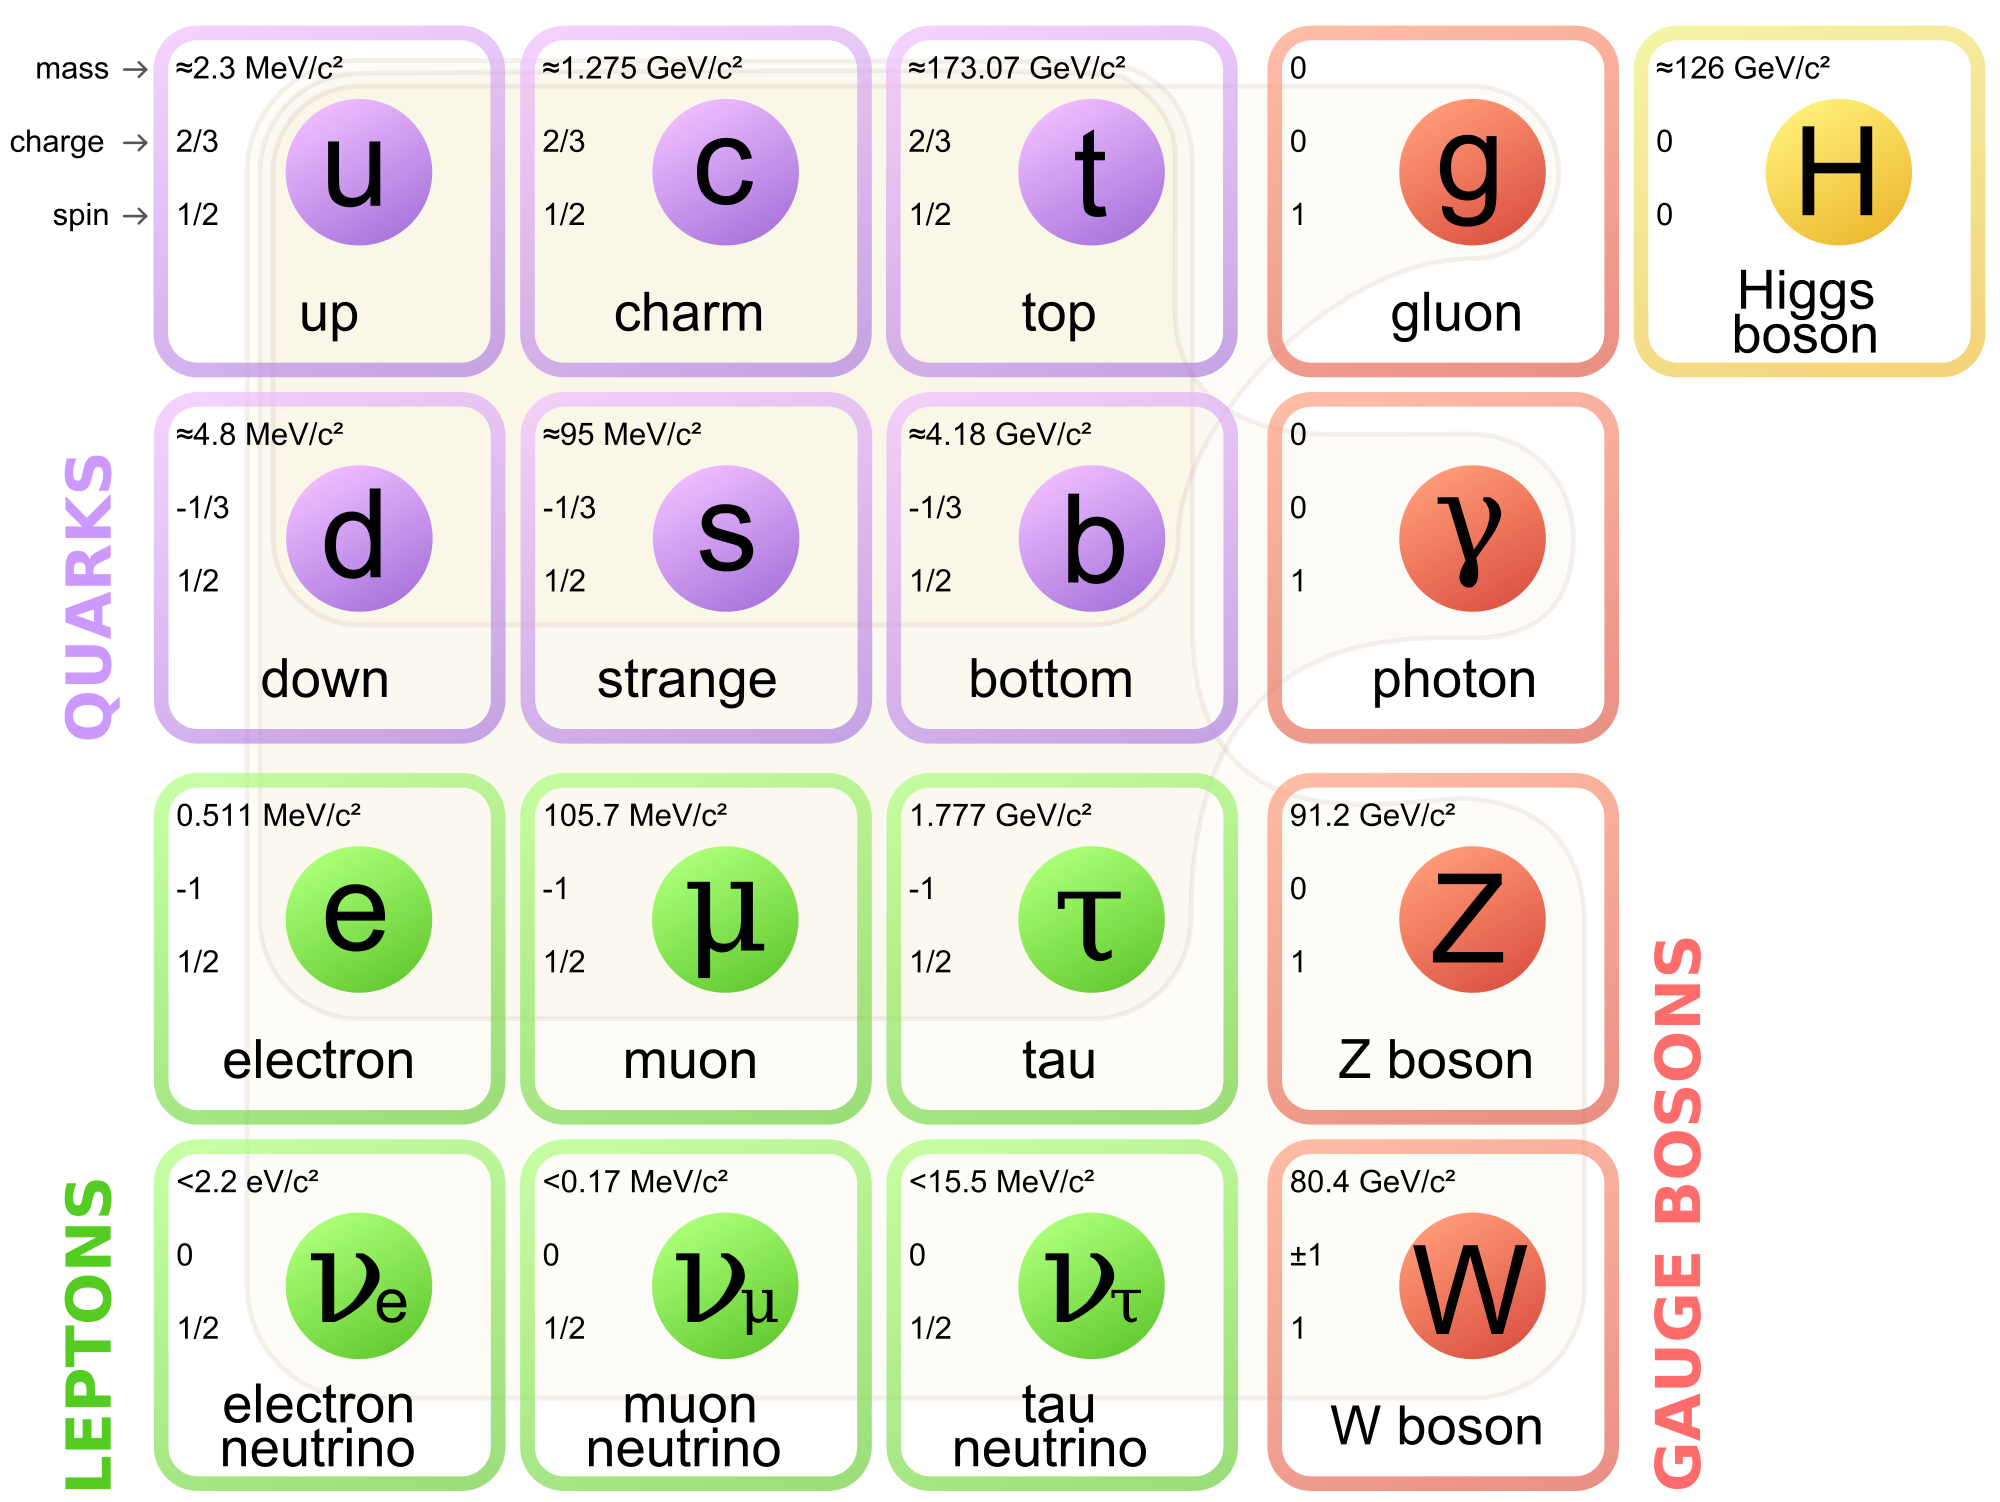
\includegraphics[scale=0.04]{Standard_Model_of_Elementary_Particles.jpg}\hspace*{0.6cm}
 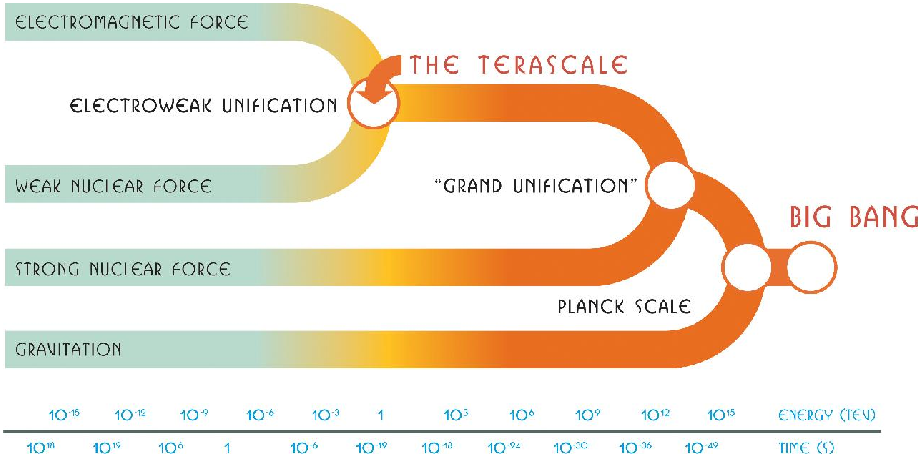
\includegraphics[scale=0.26]{energyforce.pdf}\hspace*{0.6cm}
 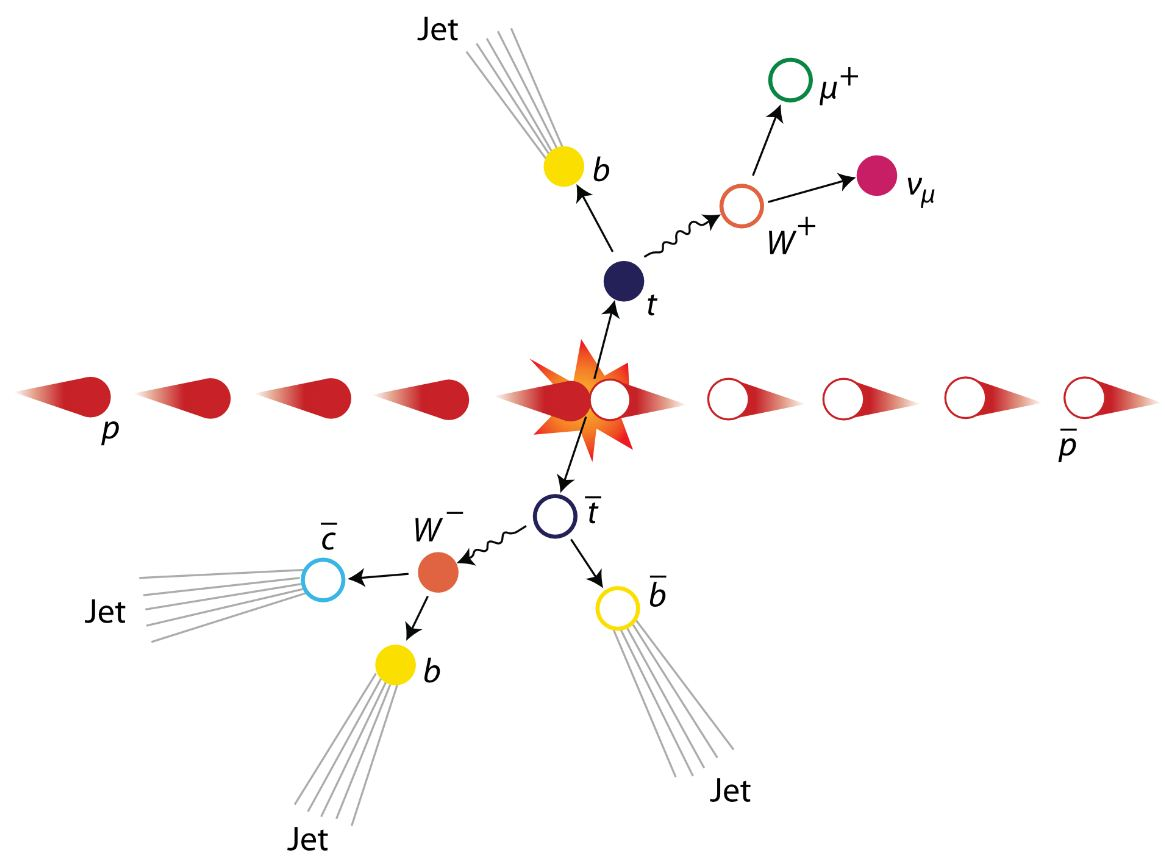
\includegraphics[scale=0.1]{top.JPG}\par\vspace*{1cm}
 \begin{picture}(0,0)
\put(40,-40){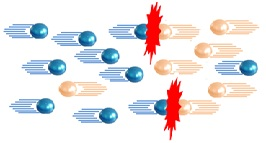
\includegraphics[scale=0.60]{3_11_1_3.jpg}}
\put(220,10){$R=\sigma \mathbf{L}$}
% \put(92,-130){\tikz\draw[red,dashed,thick] (0,0) circle (0.4);}

\put(120,-45){\color{red} 1~fb=10$^{-39}$cm$^2$}
\put(110,25){\color{red} event!}
\put(209,-8){\tikz\draw[thick,->] (-0.0,-0.0) -- (-0.5,-0.5);}
\put(170,-15){Rate of events}
\put(245,-20){\tikz\draw[thick,->] (-0.0,-0.0) -- (-0.0,-1.0);}
\put(180,-30){Interaction Cross Section	}
\put(255,-8){\tikz\draw[thick,->] (0.0,0.0) -- (0.5,-0.5);}
\put(255,-15){\textbf{Luminosity}}
\end{picture}
\end{frame}
\begin{frame}{Luminosity}
\begin{picture}(0,0)
\put(10,-45){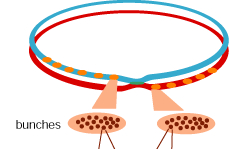
\includegraphics[scale=0.30]{circular.jpg}}
\put(40,-15){\scriptsize LEP}
\put(-10,10){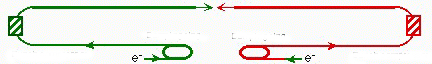
\includegraphics[scale=0.30]{linear2.jpg}}
\put(30,18){\scriptsize SLC, ILC, CLIC}
\put(125,-30){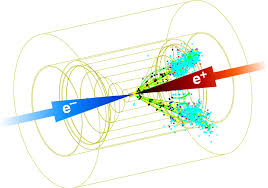
\includegraphics[scale=0.30]{linear.jpg}}
\put(210,-40){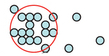
\includegraphics[scale=0.60]{paquet2.jpg}}
\put(280,-40){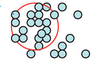
\includegraphics[scale=0.60]{paquet1.jpg}}
\put(210,-45){\tikz\draw[thick,->](0,0) -- (0,1);}
\put(210,-45){\tikz\draw[thick,->](0,0) -- (1,0);}
\put(210,-10){y}
\put(240,-45){s}
\put(235	,-25){\tikz\draw[thick,red,->](0,0) -- (1,0);}
\put(270,-20){\tikz\draw[thick,red,->](0,0) -- (-1,0);}
\end{picture}

 \begin{equation*}
 \mathbf{L} \propto \frac{f_{rep}n_b^2}{\sigma_x\sigma_y}\label{eq:lum}%\qquad\delta_{BS}\propto\frac{n_b^2E}{(\sigma_x+\sigma_y)^2}\label{eq:lum_rad}
\end{equation*}
{\tiny (@LHC, L is of the order of $10^{34}$[cm$^{-2}\cdot$s$^{-1}$])}
\hspace*{-0.7cm}
{\scriptsize
\begin{tabular}{l||c|c|c|c|c}\hline
Symbol, [Unit] & LEP & SLC & ILC & CLIC 500 GeV& CLIC 3 TeV\\\hline\hline
$E$, [TeV] &0.1046&0.050& 0.250 & 0.250 & 1.500\\
$n_b$ &$1.7\times10^{11}$&$3.3\times10^{10}$&$2\times10^{10}$&$6.8\times10^9$&$3.72\times10^9$\\
$f_{rep}$, [Hz] &$11.2\times10^3$&120&5&50&50\\
$\sigma_x/\sigma_y$, [nm]&$(200/2.5)\times10^3$&$(2.1/0.6)\times10^3$&474/5.9&202/2.3&40/1\\\hline
% E loss (Beamstrahlung) [$\Delta E/E$] &$\delta_{BS}$&-???&0.07&0.07&0.28\\
$L$, [cm$^{-2}\cdot$s$^{-1}$]&$2.1\times10^{31}$&$0.8\times10^{30}$&$1.57\times10^{34}$& $2.3\times10^{34}$&$5.9\times10^{34}$\\\hline
\end{tabular}
}
\\
Linear colliders feature \textbf{nm beam size} to achieve $10^{34}$ luminosities.
\end{frame}
\begin{frame}{Challenges for luminosity goals and nm beam size}\,
{\tiny
\begin{picture}(0,0)
\put(0,50){Beam-beam effects}
\put(-10,-20){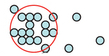
\includegraphics[scale=0.60]{paquet2.jpg}}
\put(40,0){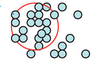
\includegraphics[scale=0.60]{paquet1.jpg}}
\put(0,-10){\tikz\draw[thick,red,->](0,0) -- (1,1);}
\put(40,0){\tikz\draw[thick,red,->](0,0) -- (-1,-1);}
 \put(140,50){Demagnify	 the beam}
 \put(115,-20){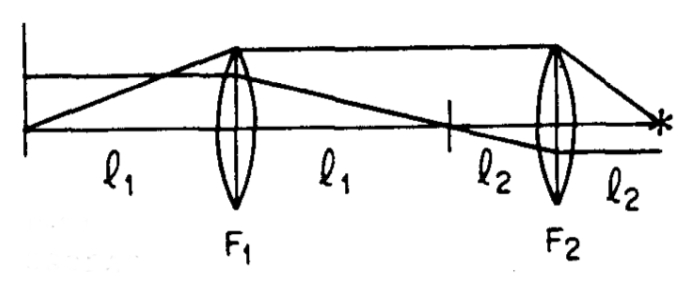
\includegraphics[scale=0.24]{telescope.jpg}}
 \put(260,50){Synchrotron radiation}
 \put(255,-20){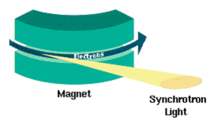
\includegraphics[scale=0.4]{220px-Syncrotron.jpg}}
 \put(0,-40){\tiny Beam positioning and stabilization}
 \put(-10,-110){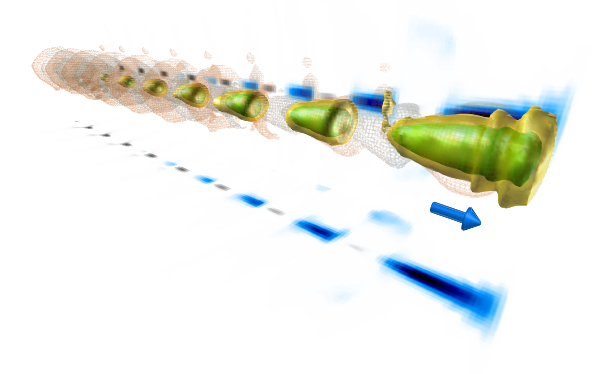
\includegraphics[scale=0.18]{bunch-self-modulated-5-arrow.jpg}}
 \put(110,-40){Small emittance beam generation and reduction}
 \put(130,-115){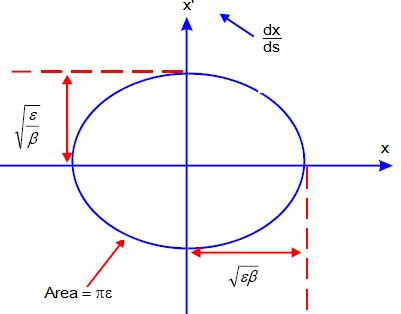
\includegraphics[scale=0.3]{4_1_2_4.jpg}}
 \put(250,-40){Small energy spread in the bunch}
 \put(270,-115){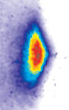
\includegraphics[scale=0.6]{I15-71-wakefield02b.jpg}}
 \put(250,-40){Small energy spread in the bunch}
\end{picture}
}
\end{frame}
\begin{frame}{Challenges for luminosity goals and nm beam size}\,
{\tiny
\begin{picture}(0,0)
\put(0,70){\scriptsize\color{blue} These are addressed in several sections of an accelerator.}
\put(0,50){Beam-beam effects}
\put(-10,-20){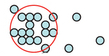
\includegraphics[scale=0.60]{paquet2.jpg}}
\put(40,0){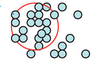
\includegraphics[scale=0.60]{paquet1.jpg}}
\put(0,-10){\tikz\draw[thick,red,->](0,0) -- (1,1);}
\put(40,0){\tikz\draw[thick,red,->](0,0) -- (-1,-1);}
\put(0,40){\scriptsize\color{blue} IP Region}
 \put(140,50){Demagnify the beam}
 \put(125,40){\scriptsize\color{blue} Final Focus Section (FFS)}
 \put(115,-20){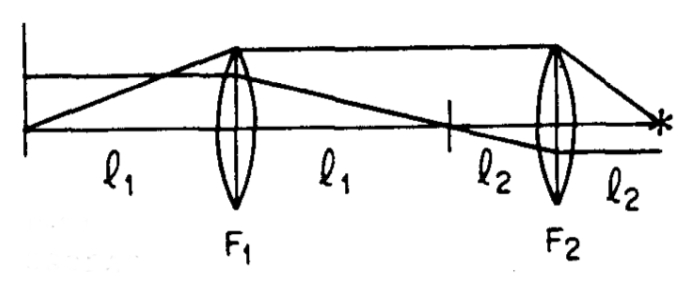
\includegraphics[scale=0.24]{telescope.jpg}}
 \put(260,50){Synchrotron radiation}
 \put(250,40){\scriptsize\color{blue} FFS, Damping Rings}
 \put(250,30){\scriptsize\color{blue} IP Region}
 \put(255,-20){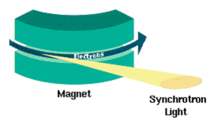
\includegraphics[scale=0.4]{220px-Syncrotron.jpg}}
 \put(0,-40){\tiny Beam positioning and stabilization}
 \put(-10,-110){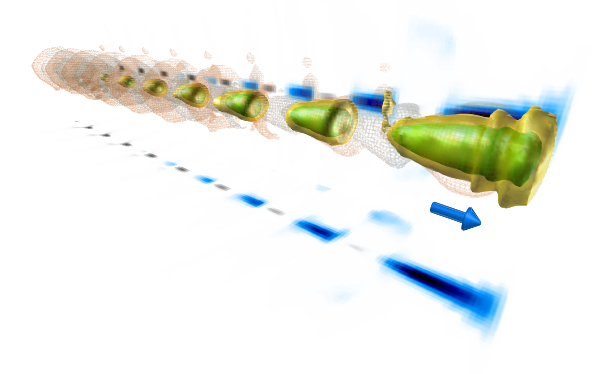
\includegraphics[scale=0.18]{bunch-self-modulated-5-arrow.jpg}}
 \put(0,-50){\scriptsize\color{blue} ALL}
 \put(110,-40){Small emittance beam generation and reduction}
 \put(130,-115){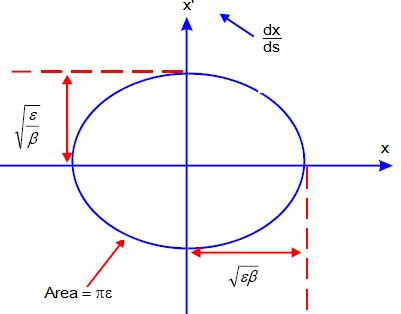
\includegraphics[scale=0.3]{4_1_2_4.jpg}}
 \put(110,-50){\scriptsize\color{blue} Damping Rings}
 \put(110,-60){\scriptsize\color{blue} Particle Source}
 \put(250,-40){Small energy spread in the bunch}
 \put(270,-115){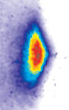
\includegraphics[scale=0.6]{I15-71-wakefield02b.jpg}}
 \put(250,-50){\scriptsize\color{blue} Particle Sources}
 \put(250,-60){\scriptsize\color{blue} LINACs}
 
\end{picture}
}
\end{frame}

\begin{frame}{Challenges for luminosity goals and nm beam size}\,
{\tiny
\begin{picture}(0,0)
\put(0,80){\scriptsize\color{blue} These are addressed in several sections of an accelerator.}
\put(0,60){\scriptsize \textbf{\underline{Main contributions} from this work to the FFS}.}
\put(0,50){Beam-beam effects}
\put(-10,-20){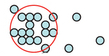
\includegraphics[scale=0.60]{paquet2.jpg}}
\put(40,0){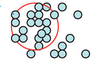
\includegraphics[scale=0.60]{paquet1.jpg}}
\put(0,-10){\tikz\draw[thick,red,->](0,0) -- (1,1);}
\put(40,0){\tikz\draw[thick,red,->](0,0) -- (-1,-1);}
\put(0,40){\scriptsize\color{blue} IP Region}
 \put(140,50){Demagnify the beam}
 \put(125,40){\scriptsize\color{blue} Final Focus Section (FFS)}
 \put(115,-20){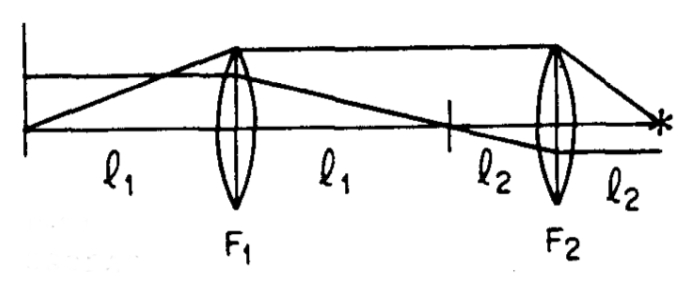
\includegraphics[scale=0.24]{telescope.jpg}}
 \put(260,50){Synchrotron radiation}
 \put(250,40){\scriptsize\color{blue} FFS, Damping Rings}
 \put(250,30){\scriptsize\color{blue} IP Region}
 \put(255,-20){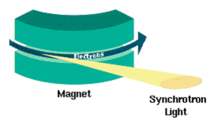
\includegraphics[scale=0.4]{220px-Syncrotron.jpg}}
 \put(0,-40){\tiny Beam positioning and stabilization}
 \put(-10,-110){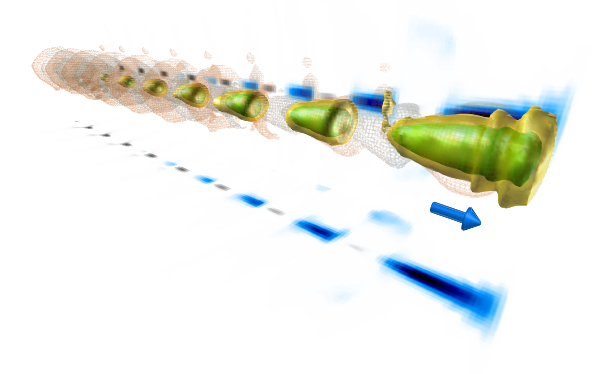
\includegraphics[scale=0.18]{bunch-self-modulated-5-arrow.jpg}}
 \put(0,-50){\scriptsize\color{blue} ALL}
 \put(110,-40){Small emittance beam generation and reduction}
 \put(130,-115){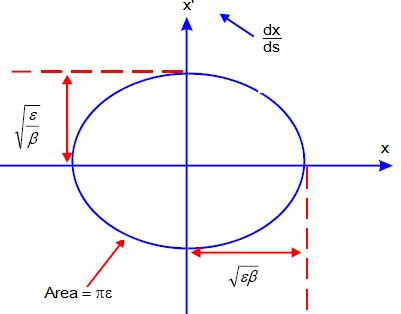
\includegraphics[scale=0.3]{4_1_2_4.jpg}}
 \put(110,-50){\scriptsize\color{blue} Damping Rings}
 \put(110,-60){\scriptsize\color{blue} Particle Source}
 \put(250,-40){Small energy spread in the bunch}
 \put(270,-115){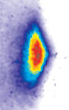
\includegraphics[scale=0.6]{I15-71-wakefield02b.jpg}}
\put(250,-50){\scriptsize\color{blue} Particle Sources}
 \put(250,-60){\scriptsize\color{blue} LINACs}
 
 \put(250,-20){\scriptsize \underline{\textbf{Oide effect}}}
 \put(120,-20){\scriptsize \underline{\textbf{Chromaticity minimization}}}
 \put(120,-30){\scriptsize \underline{\textbf{Chromaticity correction}}}
% \put(250,-20){\scriptsize \textbf{Radiation}}
\put(250,-30){\scriptsize \underline{\textbf{Rad. in bending magnets}}}
\put(0,-110){\scriptsize \underline{\textbf{IP-BPMs @ ATF2}}}
 
\end{picture}
}
\end{frame}

\begin{frame}{Sections of a Collider (CLIC 3 TeV as an example)}
 \begin{picture}(0,0)
 \put(10,-80){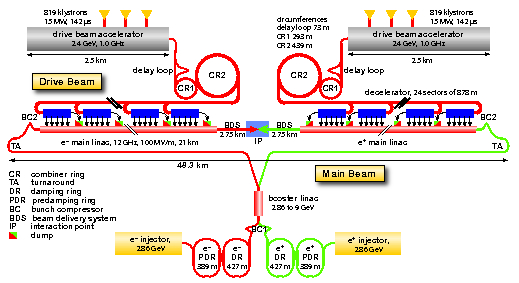
\includegraphics[scale=0.6]{Figures_CLIC-layout2012-2pub.jpg}}
% ILC
%  \put(0,70){\normalsize ILC as an example}
%  \put(220,-50){\normalsize Interaction Point (IP)}
%  \put(190,-50){\tikz\draw[thick,->](0,0) -- (-1,1);}
%  \put(170,-80){\normalsize \textbf{FFS}}
%  \put(155,-70){\tikz\draw[thick,red,->](0,0) -- (-0.5,1.5);}
%  \put(190,-70){\tikz\draw[thick,red,->](0,0) -- (0.5,2);}
%  \put(0,-90){Beam demagnification, positioning and stabilization}
%  \put(0,-100){\hspace*{0.4cm}with low effect of radiation}
% CLIC
\put(220,-40){\normalsize Interaction Point (IP)}
 \put(165,-40){\tikz\draw[thick,->](0,0) -- (-1.8,1.8);}
 \put(155,-90){\normalsize \textbf{FFS}}
 \put(150,-80){\tikz\draw[thick,->](0,0) -- (-0.5,3);}
 \put(165,-80){\tikz\draw[thick,->](0,0) -- (0.5,3);}
 \put(0,-100){Beam demagnification, positioning and stabilization}
 \put(0,-110){\hspace*{0.4cm}with low effect of radiation}
 \end{picture}
\end{frame}

% 
% \begin{frame}
% \begin{itemize}
%  \item  (Fundamental limit$\rightarrow$\textbf{Oide effect})
% \end{itemize}
% \end{frame}
% 
% \begin{frame}
% \begin{itemize}
%  \item  (Fundamental limit$\rightarrow$\textbf{Oide effect})
% \end{itemize}
% \end{frame}








% \begin{frame}{Main components}
%  \begin{itemize}
%   \item Electron/Positron sources
%   \item Damping rings
%   \item Main Linac
%   \item \textbf{Beam Delivery System (BDS)}
%  \end{itemize}
%  \centering
%  \vspace*{1cm}
% The Beam Delivery System transports the beam from the linacs to the Interaction Point~(IP).\par
% \centering
% In addition to the diagnose and collimation sections,\par in the BDS the \textbf{FINAL FOCUS SECTION (FFS)}\par is in charge of reduce (focus) the beam size (like a telescope).\\
% \end{frame}
% \begin{frame}{Motivation}
% Among the multiple effects that must be addresed because they could degrade the Luminosity, this work addressed:\par
% \begin{itemize}
%  \item (Theory) Chromaticity minimization and correction
%  \item (Theory) Synchrotron Radiation in \par \hspace*{2cm}Bending Magnets and Quadrupoles.
%  \item (Exper.) The instrumentation to diagnose errors in the lattice.
% \end{itemize}
% \end{frame}
% \begin{frame}{Beamsize}
% We are interested in the horizontal beamsize at the IP.
% \begin{multicols}{1}
% Horizontal plane
%  \begin{align*}
% %\sigma^2 &= \sigma_0^2 + \sigma_e^2 +{\color{red}\sigma_{rad}^2}\\
% \sigma^2 &= \sigma_0^2 + \sigma_i^2 +{\color{blue}	\sigma_{rad}^2}
% \end{align*}
% % Vertical plane
% %  \begin{align*}
% % \sigma^2 &= \sigma_0^2 + \sigma_e^2 +{\color{red}\sigma_{rad}^2}\\
% % \sigma^2 &= \sigma_0^2 + \sigma_e^2 +\overbrace{{\color{green}\sigma_{oide}^2}}
% % \end{align*}
% \end{multicols}
% \begin{align*}
%  \sigma_0 &\equiv \text{zero$^{\text{th}}$ order approx.}\\
%  \sigma_i &\equiv \text{result from aberrations}\\
% %  \sigma_\delta &\equiv \text{result from chromatic aberrations}\\
%  {\color{blue}\sigma_{rad}} &\equiv \text{interaction with magnets}
% \end{align*}
% Evaluated by:
% \begin{itemize}
%  \item tracking of particles
%  \item mathematical approximations
% \end{itemize}
% \end{frame}



% \begin{frame}{Beamsize}
% We are interested in the beamsize at the IP.
% \begin{multicols}{2}
% Horizontal plane
%  \begin{align*}
% \sigma^2 &= \sigma_0^2 + \sigma_g^2+\sigma_\delta^2 +{\color{red}\sigma_{rad}^2}\\
% \sigma^2 &= \sigma_0^2 + \sigma_g^2+\sigma_\delta^2 +\overbrace{{\color{blue}	\sigma_{rad}^2}}
% \end{align*}
% Vertical plane
%  \begin{align*}
% \sigma^2 &= \sigma_0^2 + \sigma_g^2+\sigma_\delta^2 +{\color{red}\sigma_{rad}^2}\\
% \sigma^2 &= \sigma_0^2 + \sigma_g^2+\sigma_\delta^2 +\overbrace{{\color{green}\sigma_{oide}^2}}
% \end{align*} 
% \end{multicols}
% \begin{align*}
%  \sigma_0 &\equiv \text{zero$^{\text{th}}$ order approx.}\\
%  \sigma_g &\equiv \text{result from geometric aberrations}\\
%  \sigma_\delta &\equiv \text{result from chromatic aberrations}\\
%  {\color{red}\sigma_{rad}} &\equiv \text{interaction with magnets}
% \end{align*}
% \end{frame}
\begin{frame}{Final Focus Section (FFS)}
 \begin{picture}(0,0)
 \put(-10,30){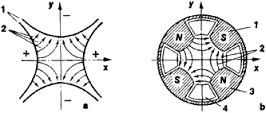
\includegraphics[scale=0.4]{quadrupolem.jpg}}
 \put(120,30){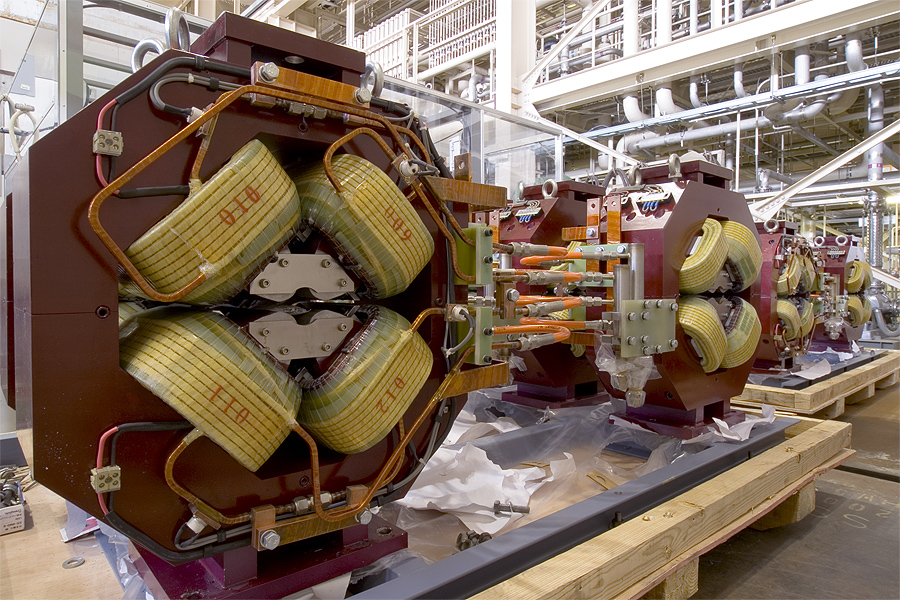
\includegraphics[scale=0.4]{20060330di-043.jpg}}
 \put(10,20){\tiny Focusing elements are magnets with 4 poles: quadrupoles}
  \put(230,25){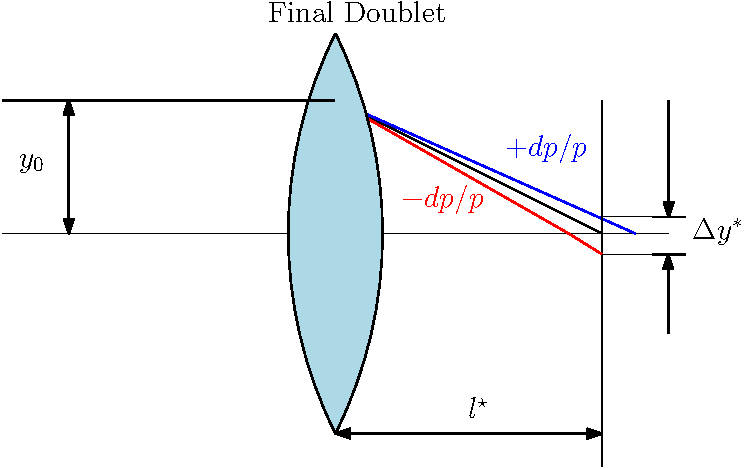
\includegraphics[scale=0.28]{chromaticity.pdf}}
  \put(220,20){\tiny Quads behave as lenses: chromatic effect}
  \put(0,0){\tiny The stronger set of lenses is the Final Doublet (FD): \textbf{QD0}, \textbf{QF1}}
  \put(0,-10){\tiny What are the distances to minimize the chromaticity ?}
 \put(0,-110){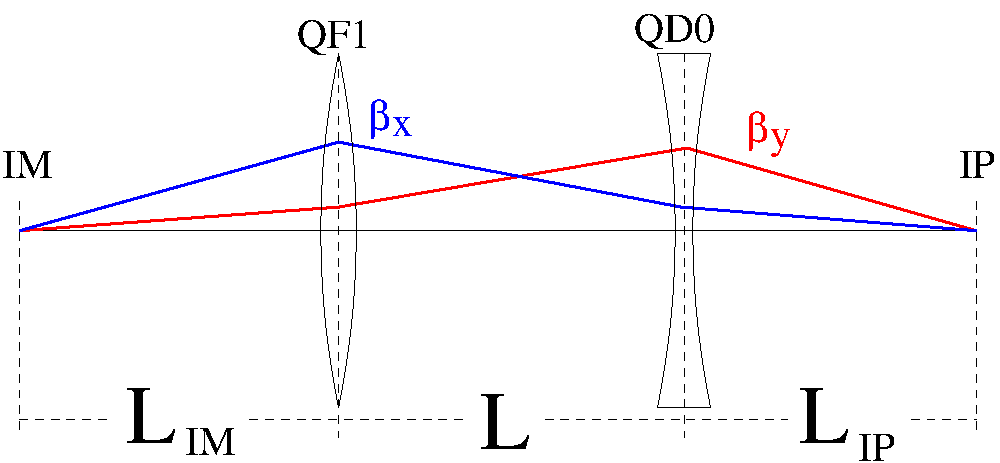
\includegraphics[angle=0,scale=0.4]{fig01.pdf}} 
 \put(140,0){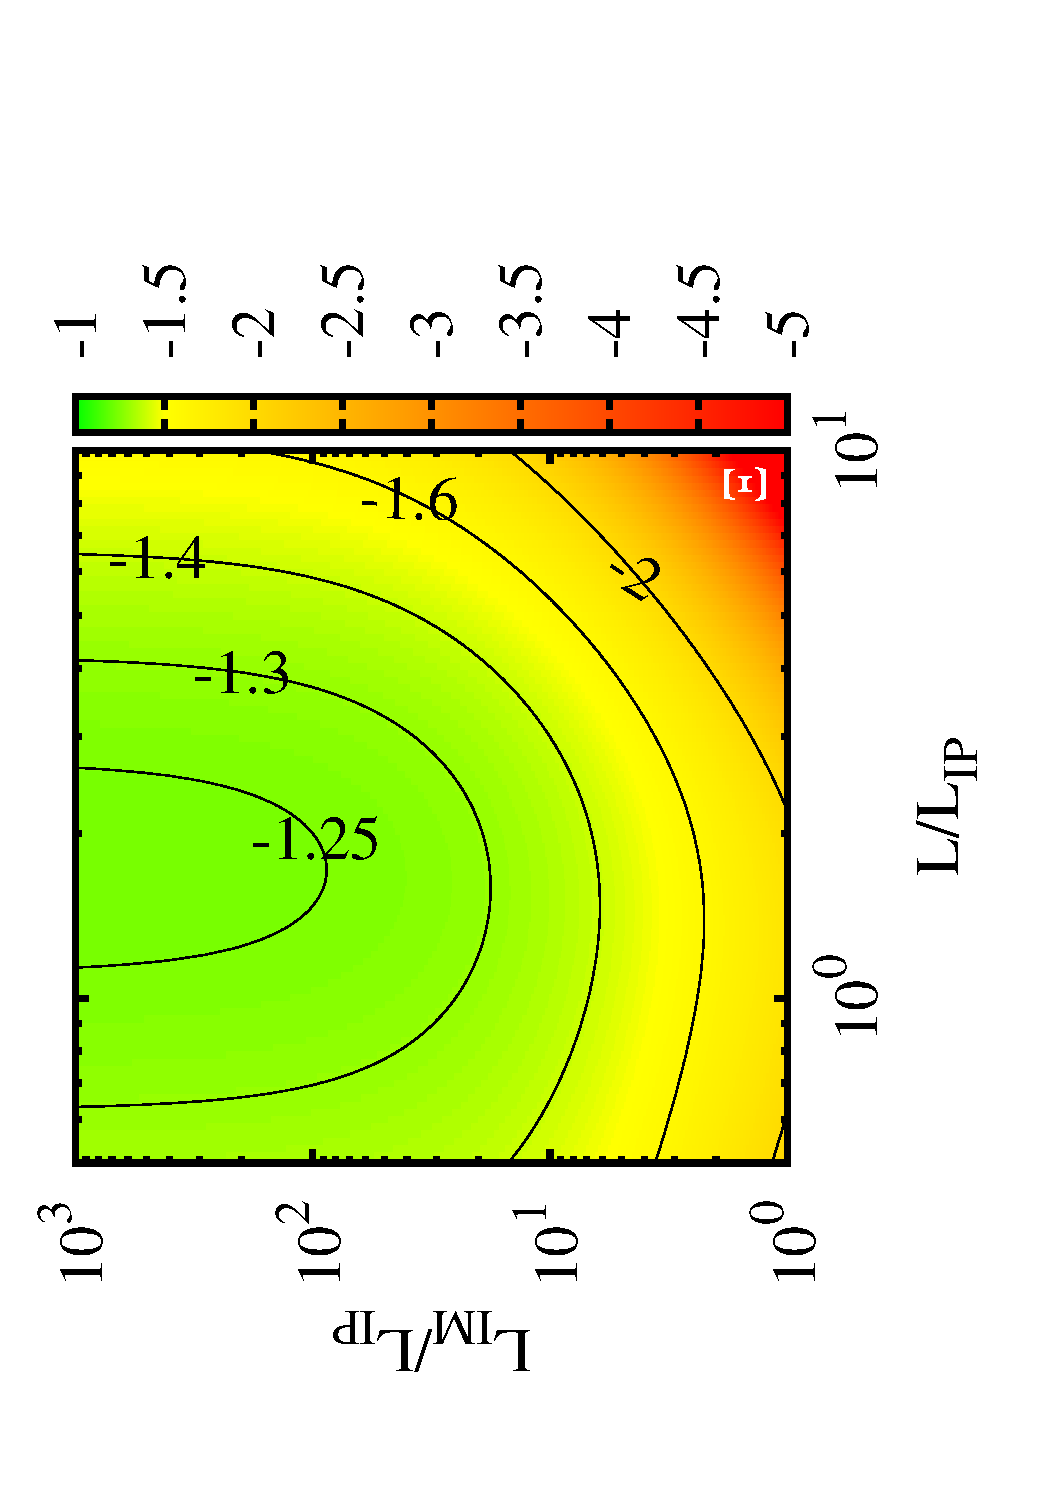
\includegraphics[angle=-90,scale=0.1]{chromHV_500GeVa.pdf}}
 \put(230,-10){\tiny \textbf{Correction of Chromatic effect}}
 \put(195,-100){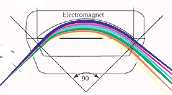
\includegraphics[angle=45,scale=0.4]{dipole.jpg}}
 \put(265,-70){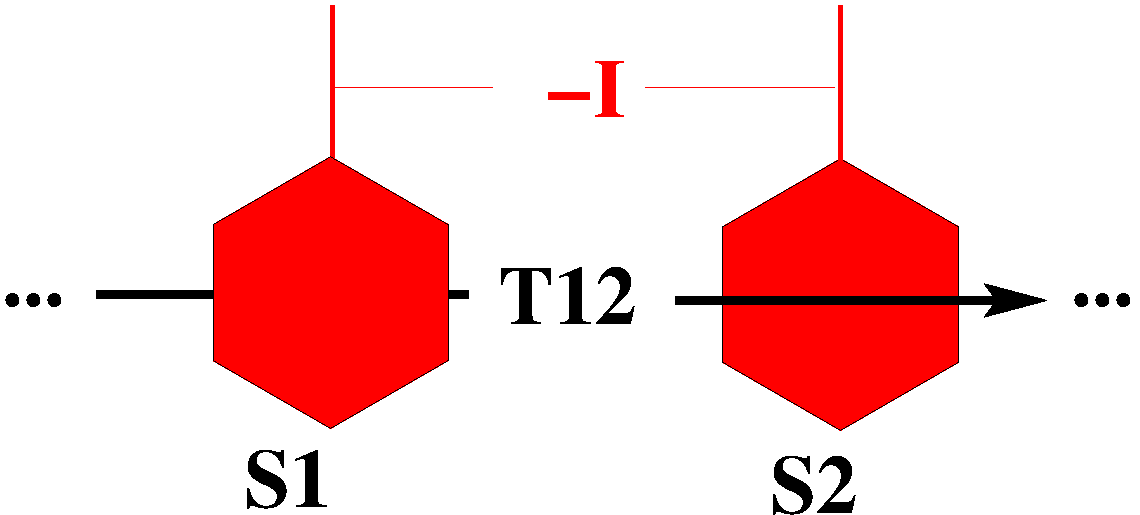
\includegraphics[angle=0,scale=0.15]{geo_cancel.pdf}}
 \put(210,-30){\tiny Bending magnets: $x=\eta_x\delta$}
 \put(280,-80){\tiny Sextupoles: $x'\propto x^2$}
 \end{picture}
\end{frame}
\begin{frame}{Chromaticity correction}
\begin{picture}(0,0)
 \put(0,80){\tiny Local chromaticity correction (Brown, 1988)}
 \put(215,90){\tiny Current \textbf{CLIC}, \textbf{ILC} and \textbf{ATF2} lines}
 \put(200,80){\tiny Local chromaticity correction (Raimondi, 2000)}
 \put(0,20){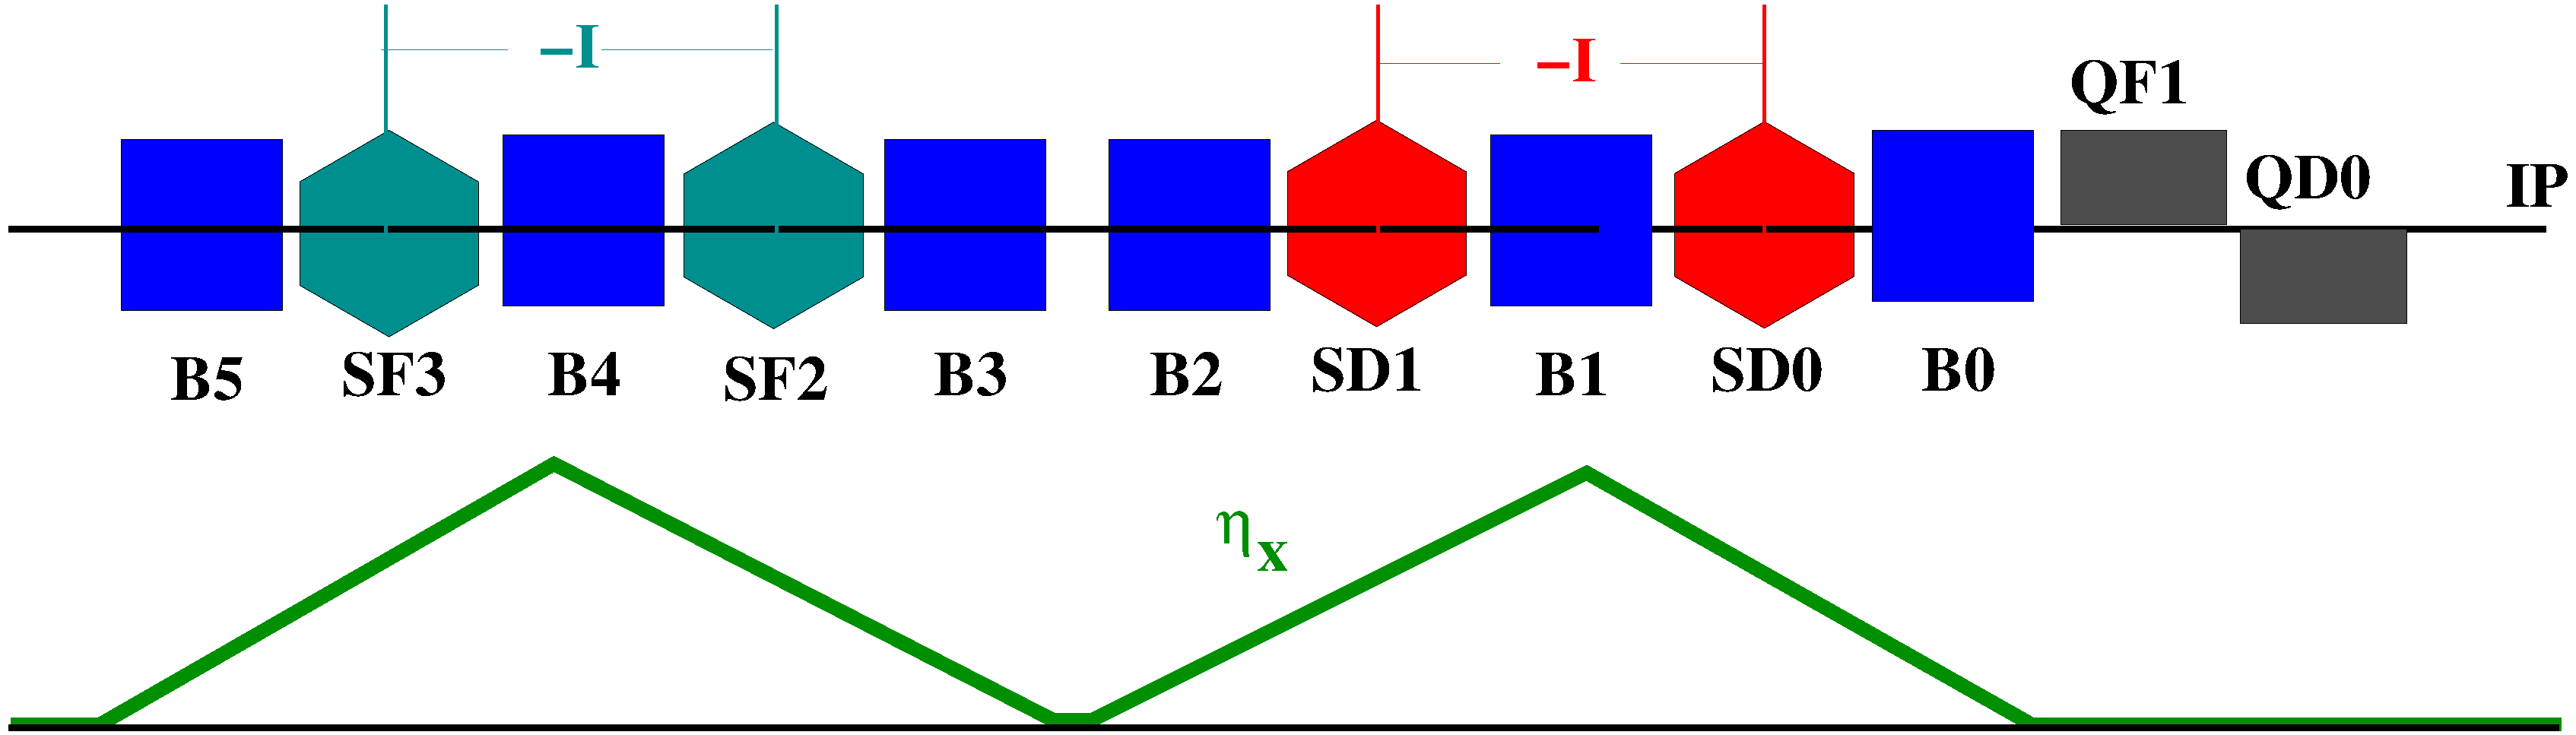
\includegraphics[scale=0.1]{nonlocalcorr2.pdf}}
 \put(210,20){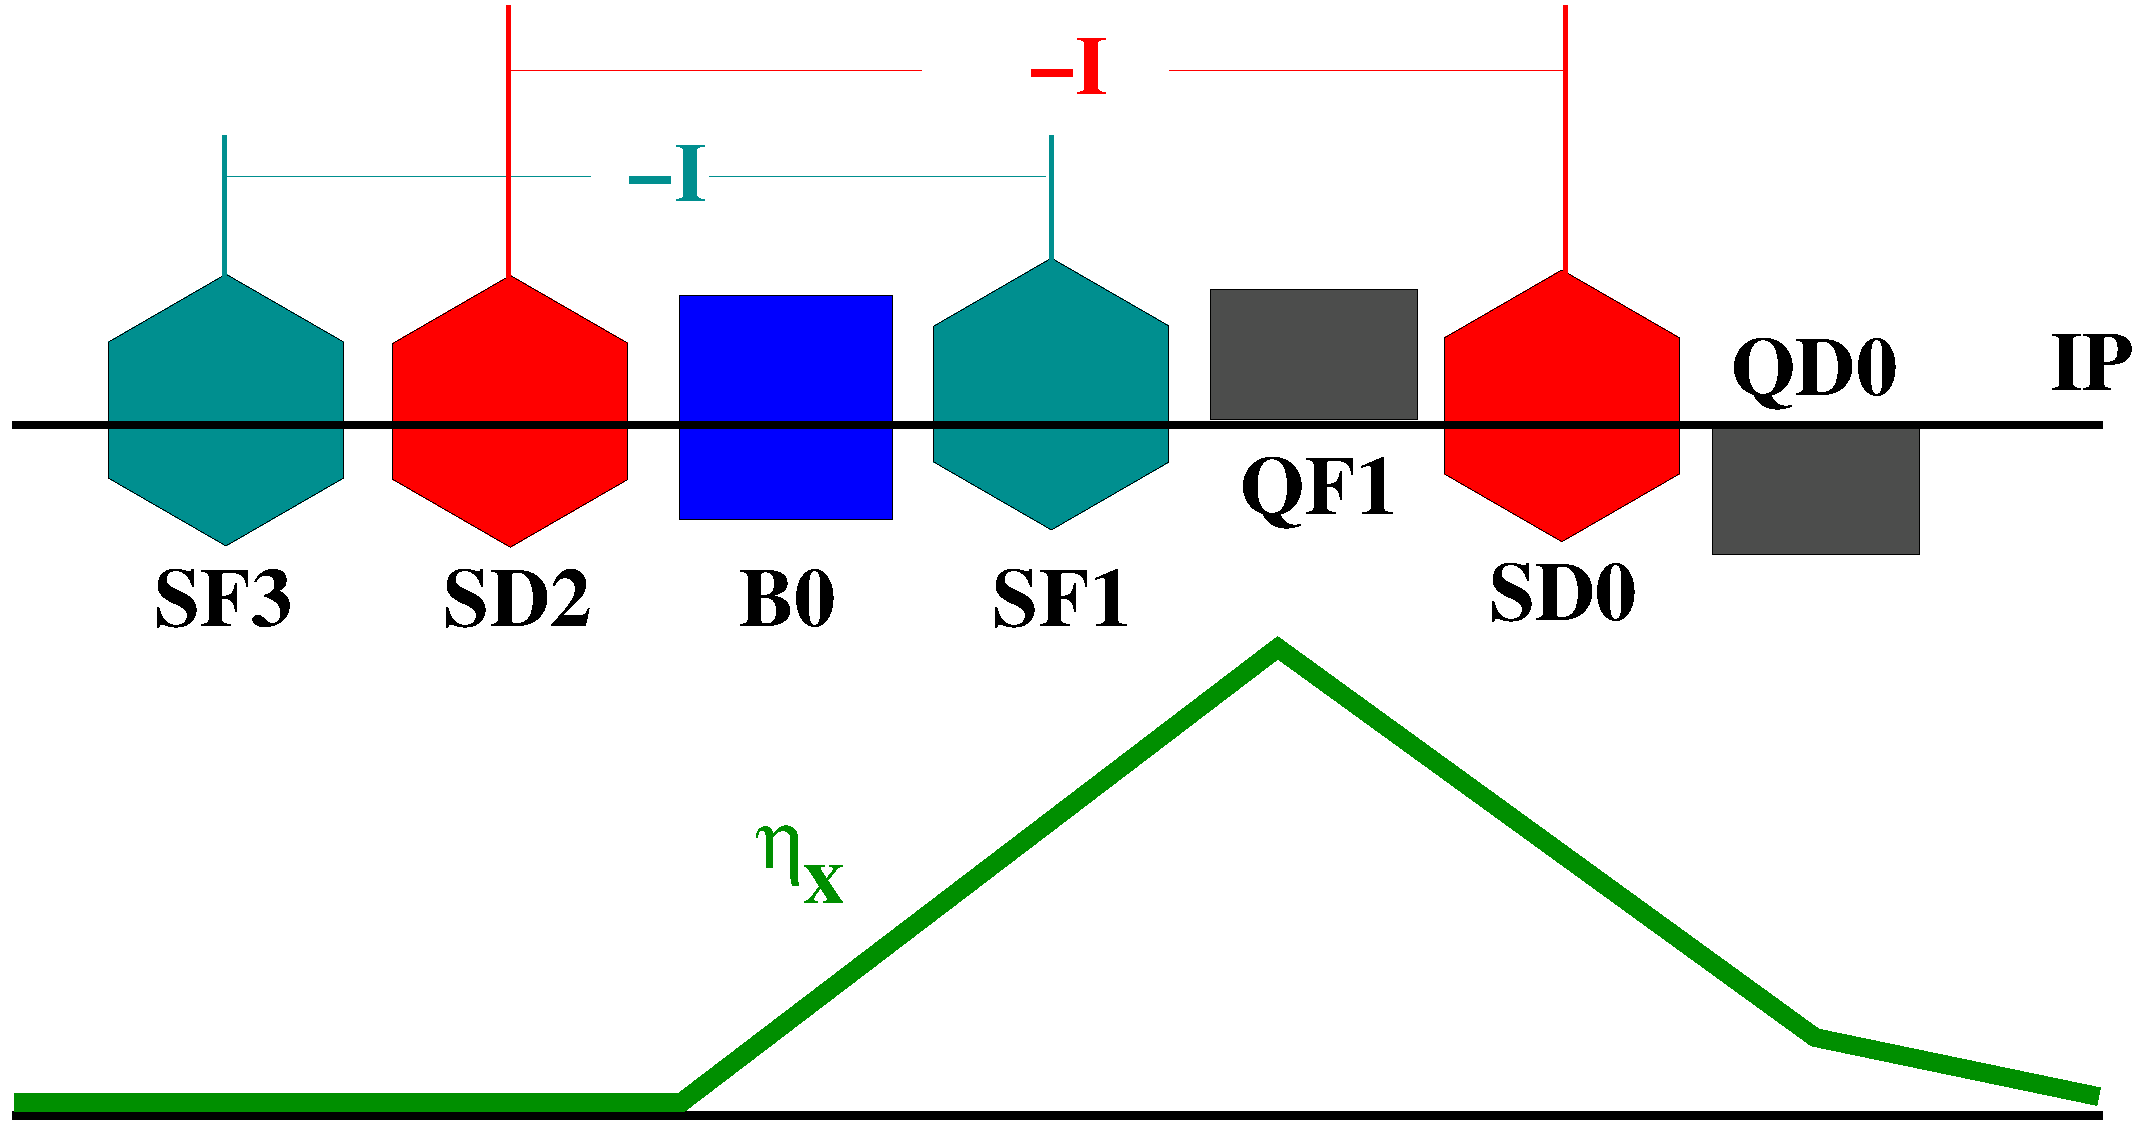
\includegraphics[scale=0.1]{localcorr2.pdf}}
 \put(-10,-75){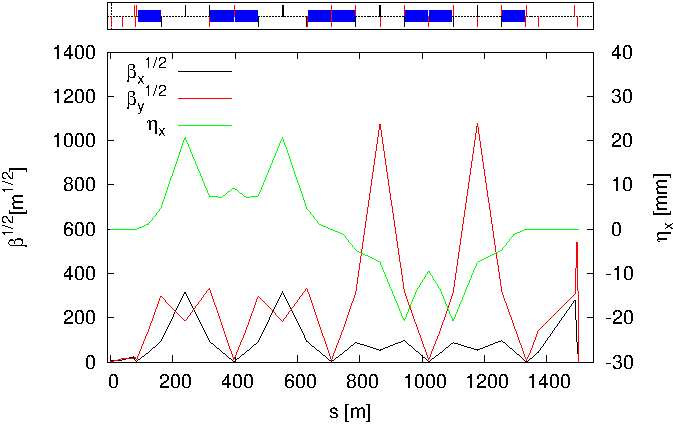
\includegraphics[scale=0.4]{CLIC3TeV_FFS_nonlocal-crop-crop.pdf}}
 \put(215,-75){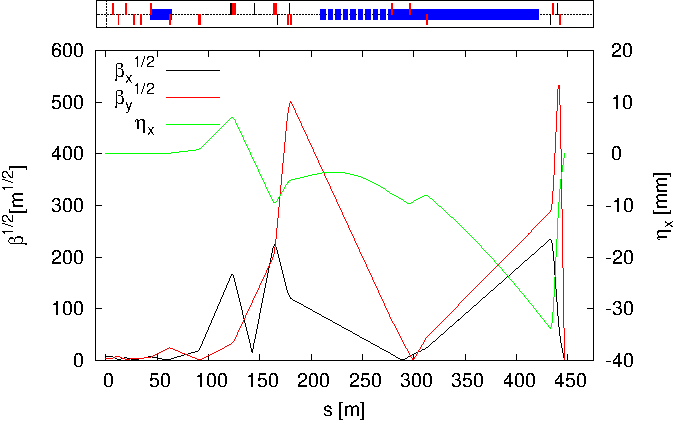
\includegraphics[scale=0.4]{CLIC3TeV_FFS_local-crop-crop.pdf}}
 \put(0,12){\tiny Easier to correct static errors, Longer line}
%  \put(0,2){\tiny Longer line}
 \put(200,12){\tiny More difficult to correct static errors, Shorter line}
%  \put(200,2){\tiny Shorter line}
\put(115,-100){\includegraphics[scale=0.08]{noninterleavedcorr2.pdf}}
\put(60,-110){\tiny Recent proposal: The non-interleaved line (Tomas, Blanco, Bambade, 2014)}
\end{picture}
\end{frame}


\section{Final focus and small beam size (CLIC)}
% \section{Oide effect}
\begin{frame}
 \color{blue}\Large Final focus and small beam size
\end{frame}
\begin{frame}
 \color{blue}\Large Radiation in bending magnets
\end{frame}
\begin{frame}{Radiation effect in bending magnets}
\begin{picture}(0,0)
  \put(-80,-50){\includegraphics[scale=0.5]{220px-Syncrotron.jpg}}
  \put(180,-170){\includegraphics[scale=0.3]{geometrysr_3a.jpg}}
  \put(190,-60){\includegraphics[scale=0.14]{Bend.jpg}}
\end{picture}
\centering
%  Higher energies have been explored with \textbf{hadron} colliders\par (\textbf{composed particles} in the SM)\par
%  \vspace*{0.5cm}
%  Precision measurements have been done with {\color{forestgreen} lepton} colliders\par ({\color{forestgreen} elemental particles} in the SM)\par
%  \vspace*{1cm}
%  .\par
Bending magnets generate energy losses
\begin{equation*}
 \Delta E\propto \frac{E^4}{\rho m_0^4}
\end{equation*}
{\tiny Energy loss is the principal limitation for circular {\color{forestgreen}lepton} colliders.\par
 The highest energy lepton collision, 209~GeV, have been reached with electron and positron coliding beams in LEP (circular tunnel of 27~km) at CERN.\par
 }\par\raggedright
 The effect on the beam size was calculated by Sands\par (SLAC/AP-47, Dec. 1985).
 \begin{equation*}
{\color{blue} x} = \sum_{i=1}^{N(T)}\Delta x_{i,total} - x_0
\end{equation*}
$N$: is the number of photons radiated (Poisson distribution)
\end{frame}





% \section{Radiation in bending magnets}
% \subsection{Theoretical model}
% \begin{frame}
%  \color{blue}\Large Radiation in bending magnets
% \end{frame}
% % \begin{frame}{Beam Radiation Model}
% 
% {\color{blue}$x$} describes the displacement of a particle at ($s=L$, e.g. IP) due to radiation, where
%  all other effects are ignored.
%  
%  \begin{equation}
% {\color{blue} x} = \sum_{i=1}^{N(T)}\Delta x_{i,total} - x_0
% \end{equation}
% \begin{itemize}
%  \item $\Delta x_{i,total} $: is the total deviation due to the $i^{\text{th}}$ photon radiated
%  \item $x_0$: is $\langle\sum_{i=1}^{N(T)}\Delta x_{i,total}\rangle$, \par \hspace*{1cm}in order to make $\langle {\color{blue}x}\rangle=0$,
%  and ${\color{blue} \sigma_{rad}^2=\langle x^2\rangle}$
%  \item $N$: is the number of photons radiated
%  \item $T$: time to cross the bending magnet
% \end{itemize}
% \end{frame}
% 
% \begin{frame}{Finding $\Delta x_i$}
% $\Delta x_i$ is the effect at $(s=L)$ due to a photon of energy $u$ radiated at $s=s_i$, therefore it has to be propagated from $s_i$ to $L$.%\footnote{Sub-index $i$ has been dropped for clarity.}
% \begin{align}
%  \Delta x_i &= (u/E) R_{16}(s_i,L) 
% \end{align}
% 
% 
% According to Sands \cite{Sands}, $N\sim Poisson$, then
% \begin{equation}
%  \sigma_N^2 = \langle N\rangle ,\qquad x_0 = \langle N\rangle\langle \Delta x_{i,total}\rangle%,\qquad {\color{blue}\sigma_{rad}^2} = \langle N\rangle \langle \overline{\Delta x}^2\rangle
% \end{equation}
% \begin{align}
% \Delta x_{i,total} &= \frac{u}{E} \sqrt{\frac{\beta_L}{\beta}}\left[\eta\cos\Delta\phi_{s_i,L}+(\alpha\eta+\beta\eta')\sin\Delta\phi_{s_i,L}\right]\\
% &= \Delta x_i + \Delta x_{i,\eta} \qquad\footnotemark\notag
% \end{align}
% \addtocounter{footnote}{-1}
% \footnote{betatron oscillation + displacement}
% \end{frame}

\begin{frame}{A generalization was required}\,
\begin{picture}(0,0)
   \put(0,-70){\includegraphics[scale=0.25]{geometrysr_3a.jpg}}
   \put(60,-15){$x=\eta\delta$}
%     \put(130,-50){\includegraphics[scale=0.24]{telescope.jpg}}
    \put(130,-60){\includegraphics[scale=0.25]{quadrupole-scan.jpg}}
    \put(250,-50){\includegraphics[scale=0.3]{4_1_2_4.jpg}}
    \put(230,-30){$\alpha$}
\end{picture}
\vspace*{2.5cm}\par
{\tiny Sands expression was valid for $\alpha=0, \eta=0$.\par
During the design process not always the focus is perfect $\alpha=0$, nor the $\eta$ is perfectly corrected.\par
}
\begin{equation*}
 {\color{blue}\sigma_{rad}^2}\approx\int E^5G^3(s)H(s)\cos^2(s)ds
\end{equation*}
It becomes:\centering
{\small
\begin{equation*}
 {\color{blue}\sigma_{rad}^2}\approx  \int \frac{E^5}{\rho^3}\left\{\sqrt{\frac{\beta_L}{\beta_s}}\left[\eta\cos\Delta\phi(s,L)+(\alpha\eta+\beta\eta')\sin\Delta\phi(s,L)\right]-\eta_L\right\}^2ds
\end{equation*}
}
{\tiny included in MAPCLASS2, lattice optimization code (published in CLIC-Note-1049)}.\par
\end{frame}


% \begin{frame}{Finding $\Delta x_i$ (cont.)}
% We could do the following approximation,
% \begin{equation}
%  \langle\Delta x_{i,total}\rangle = \cancelto{0}{\langle\Delta x_i\rangle} + \langle \Delta x_{i,\eta}\rangle = (u/E) \eta_L
% \end{equation}
% when, $\eta_L=0$ it returns exactly the same result as Sands \cite{Sands}.\par
% when, $\eta_L \neq 0$ this is the term to be substracted from $\Delta x_{i,total}$ in order to obtain the correct contribution to radiation.\par
% \begin{equation}
% {\color{blue} x} = \sum_{i=1}^{N(T)}(\Delta x_{i,total} - \langle \Delta x_{i,total}\rangle)
% \end{equation}
% 
% \textbf{Now we have an approximation when $\eta_L\neq 0$.}
% \end{frame}

% \newsavebox\radequ
% \begin{lrbox}{\radequ}%
%   \begin{minipage}{1.0\textwidth}%
%   {\scriptsize%
%  \raggedleft%
%  \vspace*{-3.4cm}
%     \begin{align*}
%     {\color{blue}\sigma_{rad}^2} &= C_2\int_0^L \frac{E^5}{\rho^3}R_{16}^2(s,L)ds\\
%     &= C_2\int_0^\theta \frac{E^5}{\rho^3}[\rho(1-\cos(\theta-\chi))]^2\rho d\chi\\
%     &={\color{marron}C_2E^5\left[\frac{1}{4}(6\theta-8\sin\theta+\sin(2\theta))\right]\qquad\footnotemark}\\
%     &={\color{marron}C_2E^5\left(\frac{\theta^5}{20}-\frac{\theta^7}{168}+\frac{\theta^9}{2880}-\frac{17\theta^{11}}{1330560}+O(\theta^{13})\right)}
%      \end{align*} 
%     }
%   \end{minipage}
% \end{lrbox}

% \begin{frame}{Result (from approximation)}
% 
% The contribution to beamsize due to radiation now can be calculated as:
% {\small
% \begin{equation*}
%  {\color{blue}\sigma_{rad}^2}\approx C_2 \int \frac{E^5}{\rho^3}\left\{\sqrt{\frac{\beta_L}{\beta_s}}\left[\eta\cos\Delta\phi(s,L)+(\alpha\eta+\beta\eta')\sin\Delta\phi(s,L)\right]-\eta_L\right\}^2ds
% \end{equation*}
% }
% \begin{itemize}
%  \item $C_2=4.13\times10^{-11}[\text{m}^2\cdot\text{GeV}^{-5}]$
%  \item $E$: is the beam energy
% \end{itemize}
% This expression was included in MAPCLASS2.\par
% It is possible to obtain a mathematical expression for one sbend magnet.
% \end{frame}

% % \subsection{One dipole}
% \begin{frame}{One dipole (theoretical expression)}
% Using $R_{16}= \rho(1-\cos\theta)$
% \begin{tabular}{p{2cm}p{10cm}}
% \includegraphics[width=4cm,height=4cm]{Bend.jpg}&\usebox{\radequ}%
% \end{tabular}
% {\scriptsize
% Theoretical expression for a drift has been also derived.
% Now, the {\color{marron}theoretical expression}, {\color{green}the approximated result} and {\color{red}tracking with PLACET} could be compared.\par
%  Some care should be taken when using {\color{marron}the expression above} due to numerical precision.\par
%  MAPCLASS2 uses on MAD-X twiss table results.\par
%  PLACET has two different radiation methods ``Default'' and ``six\_dim''.\par
%   Radiation beamsize has been normalized to the 
%  {\color{marron}theoretical value}. \par
% \addtocounter{footnote}{-1}
% \footnote{If $E$ is considered constant.}
% }
% 
% % \end{frame}
% \begin{frame}%{Results}
%  \hspace*{2.3cm}Default Synrad\hspace*{3.3cm}Flag ``-six\_dim 1''\par
%  \includegraphics[scale=0.24,angle=-90]{sigma_angle.pdf}
%  \includegraphics[scale=0.24,angle=-90]{sigma_angle_r06.pdf}\par
%   \includegraphics[scale=0.24,angle=-90]{sigma_Lbend.pdf}
%  \includegraphics[scale=0.24,angle=-90]{sigma_Lbend_r6.pdf}\par
% \end{frame}

\begin{frame}{Comparing theory with the tracking code PLACET}
\hspace*{2.2cm}PLACET 0.99.01\hspace*{2.8cm}PLACET 0.99.02
 \includegraphics[scale=0.24,angle=-90]{sigma_Ldrift.pdf}
 \includegraphics[scale=0.24,angle=-90]{sigma_Ldrift_r6.pdf}\\
 \centering\vspace*{1cm}
 1) The lattice optimization of the line's optics now includes radiation!\par
 2) This lead to an improvement in the tracking code calculations!\par
\end{frame}

\newcommand{\twisslogo}{
  \setlength{\TPHorizModule}{1pt}
  \setlength{\TPVertModule}{1pt}
   % textblock{}{x,y}: pos(x) = leftUpperCorner + (x * \TPHorizModule), pos(y) = leftUpperCorner - (y * \TPVertModule)
%   \begin{textblock}{1}(5,205)
  \begin{textblock}{1}(200,80)
   Twiss
  \end{textblock}
  }

  \newcommand{\ptctwisslogo}{
  \setlength{\TPHorizModule}{1pt}
  \setlength{\TPVertModule}{1pt}
   % textblock{}{x,y}: pos(x) = leftUpperCorner + (x * \TPHorizModule), pos(y) = leftUpperCorner - (y * \TPVertModule)
%   \begin{textblock}{1}(5,205)
  \begin{textblock}{1}(200,190)
   ptc\_twiss
  \end{textblock}
  }
  
% \begin{frame}
% %    \hspace*{2.3cm}Twiss\hspace*{3.3cm}Flag ``ptc\_twiss''\par
%  \includegraphics[scale=0.24,angle=-90]{sigma_angle_r6_twiss.pdf} \par
%  \includegraphics[scale=0.24,angle=-90]{sigma_angle_r06.pdf}
%  \twisslogo
%  \ptctwisslogo
% \end{frame}


% \begin{frame}{Results (cont.)}
% Including a drift in front of the bending magnet.
% \begin{tabular}{p{3.5cm}p{10cm}}
% \includegraphics[angle=-90,scale=0.20]{Bend+drift2.jpg}&\includegraphics[angle=-90,scale=0.23]{sigma_Ldrift.pdf}%
% \end{tabular}
% 
%  In this case the radiation beamsize has been normalized to {\color{green}the approximated result}\par
% \textbf{Agreement between 80\% and 90\%}
% \end{frame}

% \section{Optimization Results and Conclusions}
% \subsection{Optimization}
% \begin{frame}{Optimization}
% The total length is fixed.
%  \includegraphics[width=10cm,height=3cm]{dipolesect.jpg}\par
% Total angle distribution will be changed to minimize ${\color{blue}\sigma_{rad}}$, under the following constraints:
% \begin{itemize}
%  \item $\eta_x(IP) = 0$
%  \item $\eta'_x(IP) = $constant value
% \end{itemize}
% \end{frame}
% \begin{frame}{Result}
% \begin{tabular}{lcc}
%  & $\sigma_{bef}$[nm]&$\sigma_{aft}$[nm]\\
% CLIC 3TeV & 46.28 & {\color{red}46.3}
% % CLIC 500GeV & 215.2 & -\\
% % ILC 500GeV & 477.2 & -\\
% \end{tabular}
% \begin{center}
%  \includegraphics[scale=0.31,angle=-90]{eta_opt.pdf}
% \end{center}
% %  \begin{textblock}{1}(50,60)
% %   
% %  \end{textblock}
% %  \tiny
% %    \includegraphics[height=1.6cm,keepaspectratio]{LAL.jpg}
% 
% 
%   
% \end{frame}
% % \begin{frame}
% %  However, beamsize is composed by
% %  \begin{equation*}
% %   \sigma^2 = \sigma_0^2 + \sigma_g^2+\sigma_\delta^2 +{\color{blue}	\sigma_{rad}^2}
% %  \end{equation*}
% % and, dispersion is used in the lattice to correct geometrical ($\sigma_g$) and chromatic ($\sigma_\delta$) aberrations (see \cite{Renier}).\par
% % It is required to include sextupoles in the optimization.
% % \end{frame}
% % \begin{frame}\hspace*{-1cm}
% %  \includegraphics[width=7cm,height=12.7cm,angle=-90]{im02.png}
% %  \begin{textblock}{1}(50,180)
% %  \tiny
% % %    \includegraphics[height=1.6cm,keepaspectratio]{LAL.jpg}
% % \begin{tabular}{lcc}
% %  & $\sigma$[nm] & ${\color{blue} \sigma^2_{bends}}[10^{-16}$m$^2$]\\
% % CLIC 3TeV & 46.3&5.54\\
% % CLIC 500GeV & 215.3&1.94\\
% % ILC 500GeV & 477.6&3.56\\
% % \end{tabular}
% % 
% %   \end{textblock}
% % \end{frame}

% \subsection{Conclusion}
% \subsection{Low number of photons}
% \begin{frame}{Low number of photons}
% Average number of photons emitted is
% \begin{align}
%  \langle N\rangle&= \frac{1}{c} \int_0^L ds \int_0^\infty du\; n(u,s)\\
%  &\approx C_1E\theta\qquad\qquad\qquad;C_1=20.61\text{[GeV]}^{-1}
% \end{align}
% \par
% \includegraphics[scale=0.24,angle=-90]{sigma_angle_r06.pdf}
% \includegraphics[scale=0.22,angle=-90]{sigma_Bfix5e-3T.pdf}
% 
% \end{frame}

% \begin{frame}
% %  \begin{array}{cc}
% %  \hspace*{2.3cm}Default Synrad\hspace*{3.3cm}Flag ``-six\_dim 1''\par
%  \includegraphics[scale=0.24,angle=-90]{histogram1e-2.pdf}
%  \includegraphics[scale=0.24,angle=-90]{histogram1e-3.pdf}\par
%   \includegraphics[scale=0.24,angle=-90]{histogram1e-4.pdf}
%  \includegraphics[scale=0.24,angle=-90]{histogram1e-5.pdf}\par
% %  \end{array}
% 
% \end{frame}

% % \subsection{Conclusions}
% \begin{frame}{Conclusions}
% \begin{itemize}
%  %\item The lattice was already optimized to balance between correction of aberrations and radiation effects. Differences in beamsizes are minimum.
%  \item Mapclass2 agrees with theory, some care should be taken with twiss file.
%  \item ``six\_dim'' in PLACET radiation model is more accurate than default radiation calculation. Both shows differences with theoretical model for bends causing low photon emission.
%  \item Theoretical model for low photon emission stills in check.
% 
% %  \item 
% %  \item Any region with large betas could be used to place bending magnets with minimum effect on radiation.
% %  \item Next optimizations will include more parameters.
% \end{itemize}
% 
% \end{frame}
























\begin{frame}
 \color{blue}\Large Oide effect
\end{frame}
\begin{frame}{Oide effect}
Radiation in a focusing magnet changes the energy of the particle and limits the focusing effect.\par
\centering
 \includegraphics[scale=0.4,angle=0]{Oide.pdf}\\
{\tiny {\color{blue} Designed particle trajectory}, {\color{red} trajectory of a particle due to radiation in the quadrupole}}.\par
\end{frame}
\begin{frame}{Oide limit}
% The beam size will be : 
%  \begin{equation*}
%   \sigma_y^2 = \beta_y^*\epsilon_y + c_1\gamma^5F(\sqrt{K}L,\sqrt{K}L^*)\left(\frac{\epsilon_y}{\beta_y^*}\right)^\frac{5}{2}
%  \end{equation*}
The minimum beam size is independent of energy\par (PhysRevLett.61.1713, 1988).
\begin{equation*}
 \sigma^*_{y \text{ min}} = c_2\left[F(\sqrt{K}L,\sqrt{K}L^*)\right]^\frac{1}{7}(\epsilon_{Ny})^\frac{5}{7}
\end{equation*}
{\scriptsize
\begin{table}[hbt]\hspace*{-0.7cm}
\begin{tabular}{l||c|c|c||c|c|c|c|c||c|c}\hline
Lattice &$\epsilon_N$& $\gamma$& $\sigma_0$&$k$&$L$&$L^*$& $F$ & $\sigma_{oide}$&$\sigma$&$\sigma_{min}$\\
 &(nm)&($10^3$)&(nm)&(m$^{-2}$)&(m)&(m)&&(nm) &(nm)&(nm)\\\hline\hline
CLIC 3 TeV & 20 & 2935.0 & 0.70 & 0.116 & 2.73 &3.5&  4.086  & 0.85 & 1.10& 1.00 \\
CLIC 500 GeV & 25 & $\;\;$489.2 & 2.3 & 0.077 & 3.35 &4.3& 4.115 & 0.08 & 2.3 & 1.17\\
ILC  500 GeV & 40 & $\;\;$489.2 & 5.7 & 0.170 & 2.20 &4.3& 9.567 & 0.04 & 5.7 & 1.85\\\hline
\end{tabular}\label{tabSigmas}
\end{table}\par
}
\end{frame}
\begin{frame}{Oide in CLIC 3TeV}
%  The current particle distribution in CLIC 3TeV at the IP.
 \includegraphics[scale=0.2,angle=-90]{plotxrad.pdf}
 \includegraphics[scale=0.2,angle=-90]{plotyrad.pdf}\\\centering
 \includegraphics[scale=0.2,angle=-90]{plotxyrad.pdf}\par
 The ideal would be to remove $\Delta y = y_\text{rad} -y_0$.\par
\end{frame}
\begin{frame}{$\Delta y$ due to radiation}
Oide averages over $u,s,y,y'$, obtaining $\langle \Delta y \rangle = 0$.\par
%This position variation is not coherent with any beam parameter, \textbf{but} its 
But this result hides a correlation between $\Delta y, y'$:\par
\begin{equation*}
 \langle\Delta y (y'_0)\rangle = \frac{2}{3}r_e\gamma^3G(\sqrt{K}L,\sqrt{K}L^*)(y'_0)^3
\end{equation*}
% $r_e$ is the clasical electron radius and
% {\scriptsize
% \begin{equation*}
%  G(\sqrt{K}L,\sqrt{K}L^*)=\int_0^{\sqrt{K}L}(\sin\phi+\sqrt{K}L^*\cos\phi)^2\int_0^\phi (\sin\phi'+\sqrt{K}L^*\cos\phi')^2 d\phi'd\phi
% \end{equation*}
% }
\par\centering\vspace*{-0.5cm}
\includegraphics[scale=0.25,angle=-90]{plotdyrad.pdf}\par\centering
{\scriptsize For CLIC 3 TeV parameters it is possible to substract 10\% of the Oide effect.}\par
\end{frame}
% \subsection{Corrector}
\begin{frame}{Corrector}
A pair of correctors is added to the strong focusing in order to mitigate the radiation effect.\par
\centering
\includegraphics[scale=0.3,angle=0]{Oide2.pdf}\par\raggedright
{\color{blue}nominal trajectory}: the kick in C1 must cancel the kick in C0.\par
{\color{red}all particles that radiate}: the difference in kicks should cancel $\Delta y$.\par\vspace*{1cm}
% Procedure:\par
% \begin{itemize}
%  \item Scan the best position and gradient ($s,k$) for C0.
%  \item Set C1 at QD0 input to cancel the effect of C0.
% \end{itemize}
\end{frame}
% \begin{frame}{Corrector (cont.)}
% \centering
% \includegraphics[scale=0.3,angle=-90]{plotdyradfit.pdf}\par 
% Two sets of corrector could be used :
% \begin{itemize}
%  \item For the linear fit : Quadrupoles (QD00,QD01)
%  \item For the cubic fit : Octupoles (OD0,OD1)
% \end{itemize}
% \end{frame}
% \begin{frame}{Corrector (quad, oct)}
% \begin{columns}[T]
% \begin{column}{.48\textwidth}
% \centering
%    Quadrupoles\par\hspace*{-0.5cm}
%    \includegraphics[scale=0.25,angle=-90]{plotdyradquad.pdf}\par
%    Beam size reduction\par$3.0\%\pm0.7$
% \end{column}
% \hfill
% \begin{column}{0.48\textwidth}
% \centering
%    Octupoles\par\hspace*{-0.7cm}
%    \includegraphics[scale=0.25,angle=-90]{plotdyradoct.pdf}\par
%    Beam size reduction\par$4.3\%\pm0.7$
% \end{column}
% \end{columns}
% \end{frame}
% \begin{frame}{Oide+Oct in CLIC 3TeV}
%  The current particle distribution in CLIC 3TeV at the IP.
%  \includegraphics[scale=0.2,angle=-90]{plotxradoct.pdf}
%  \includegraphics[scale=0.2,angle=-90]{plotyradoct.pdf}\\\centering
%  \includegraphics[scale=0.2,angle=-90]{plotxyradoct.pdf}\par
%  Beam size reduction of 4\% !\par
% \end{frame}
% \subsection{Limitation}
\begin{frame}{Result}\,\vspace*{-2.6cm}
{\tiny 
 A 4\% of beam size reduction was possible for CLIC 3 TeV (6\%$\sim$7\% of Oide effect reduction).\par
 Why it was not possible to reduce the correlation even more ?}\par\centering\vspace*{-0.0cm}
 {\scriptsize
 \begin{tabular}{c||c|c|c|c||c|c||c|c}\hline
& \multicolumn{2}{c|}{OD1} &\multicolumn{2}{c||}{OD0} & $\sigma_x$ & $\sigma_y$ & $L_{tot}$ & $L_{peak}$\\
& $l$ [m] & $k_3$ [m$^{-4}$] & $l$ [m] & $k_3$ [m$^{-4}$] &  [nm] & [nm] & \multicolumn{2}{c}{[$10^{34}$cm$^{-2}\cdot$ s$^{-1}$]}\\\hline\hline
NO RAD & 0.01 & 0 & 0.01 & 0 & 47.45 & 0.69 & 7.7 & 2.9\\
RAD    & 0.01 & 0 & 0.01 & 0 & 47.45 & 1.18 & 7.5 & 2.7 \\
RAD    & 0.01 & 0 & 0.01 & -3900 & 47.45 & 1.13 & 7.4 & 2.7 \\
RAD    & 0.01 & 1502 & 0.01 & -3900 & 47.45 & 1.17 & 7.1 & 2.7 \\\hline
%NO RAD & 0.01 & 0 & 0.01 & -3900 & 47.42 & 0.77 & - & -\\
%NO RAD & 0.01 & 1502 & 0.01 & -3900 & 47.42 & 0.75 & - & -\\\hline
\end{tabular}
}\par
\begin{picture}(0,0)
 \put(0,0){\includegraphics[angle=-90,scale=0.20]{lattice_CLIC_3TeVFD.pdf}}
 \put(0,-10){\tiny (to be submitted to PRST-AB next week).}
 \put(150,-40){\tiny ($\beta_y/\beta_x$) ratio needs to be equal for both correctors.}
 \put(150,-50){\tiny The phase advance between correctors.}
\end{picture}
% %  \includegraphics[scale=0.3,angle=0]{Oide2.pdf}\par\raggedright
%  \begin{itemize}
% %   \item C0 adds very little to radiation. But at some point the radiation in C1 starts to be important. It might be possible to scan  C1 ($s,k$) to find a place where it radiates less.
% %   \item Even with perfect C1 to C0 correction there will be a limit when radiation will affect the Horizontal plane. Here the target was set to less than 1\% of horizontal beam size increase.
%  \item The cancellation depends on $\beta_y/\beta_x$ ratio and phase advance.
%   \item Mean correlation could be reduced to a minimum as \par there is not correlation per each particle
%  \end{itemize}
\end{frame}

% % \subsection{Conclusions}
% \begin{frame}{Conclusions}
% \begin{itemize}
% \item Radiation in the final quad sets a limit on the vertical beamsize, this is called Oide effect
% \item Even if the mean value of the trajectory change is zero, there is a correlation between the change in trajectory and the angle at the IP due to the energy change.
% \item This correlation is reduced by correctors before and after QD0. The best result yet has been with octupoles giving a vertical beam size reduction of $4.3\%\pm0.7$
% \end{itemize}
% \end{frame}

% \section*{References}
% \begin{frame}{References}
%  \begin{thebibliography}{6}
%   \bibitem{Oide} K. Oide. Synchrotron-Radiation Limit on the Focusing of Electron Beams.	Phys. Rev. Lett. 61  Issue 15, Oct, 1988. Pages 1713 - 1715.
% \bibitem{Xu} Xu, G. General conditions for self-cancellation of geometric aberrations in a lattice structure. PRST-AB 8,104002, 2005.
% \bibitem{Placet} PLACET. https://savannah.cern.ch/projects/placet/% Link consulted 2013.04.17
% \bibitem{Wolfram} http://www.wolframalpha.com/% Link consulted 2015.01.07
% %  \bibitem{Renier} Renier, Ives. Implementation and validation of the linear collider final focus prototype : ATF2 at KEK (Japan). Doctoral Thesis, LAL10-91. June 2010.
%  \end{thebibliography}
% \end{frame}
% \begin{frame}{Additional slide}
% Dispersion function
% \begin{equation*}
% \begin{pmatrix}
%  \eta(s_2)\\
%  \eta'(s_2)\\
%  1
% \end{pmatrix}
% =
% \begin{pmatrix}
%  C(s_1,s_2) & S(s_1,s_2)& R_{16}(s_1,s_2)\\
%  C'(s_1,s_2) & S'(s_1,s_2) & R_{26}(s_1,s_2)\\
%  0 & 0 &1
%  
% \end{pmatrix}
% \begin{pmatrix}
%  \eta(s_1)\\
%  \eta'(s_1)\\
%  1
% \end{pmatrix}
% \end{equation*}
% PLACET error bars
% \begin{align*}
%  f&= \frac{x_{rad}^2-x_{norad}^2}{x^2_0}\\
%  \delta f &= \frac{2}{\sqrt{N}}\frac{(x^2_{rad}+x^2_{norad})}{x_0^2}
% \end{align*}
% \end{frame}
% 



% \section{Oide effect}
% \subsection{Introduction}
% \begin{frame}
%  \centering\includegraphics[width=8cm,height=4cm]{Oidea.jpg}
%  \begin{equation*}
% {\color{green} \sigma_{oide}^2} =\frac{110}{3\sqrt{6\pi}}r_e\lambda_e\gamma^5 {\color{forestgreen}F(\sqrt{K}L,\sqrt{K}L^*)}\left(\frac{\epsilon_y}{\beta^*_y}\right)^{5/2}
% \end{equation*}
% {\tiny
% \begin{equation*}
%  {\color{forestgreen}F(\sqrt{K}L,\sqrt{K}L^*)}=\int^{\sqrt{K}L}_0 |\sin\phi+\sqrt{K}L^*\cos\phi|^3\left[\int^\phi_0(\sin\phi'+\sqrt{K}L^*\cos\phi')^2d\phi'\right]^2d\phi
% \end{equation*}
% Equation derived by \cite{Oide}.
% }
% 
% \end{frame}
% \begin{frame}{Two approaches}
%  For a given $L^*$, what is the gradient K that minimizes ${\color{forestgreen}F(\sqrt{K}L,\sqrt{K}L^*)}$?
%  \begin{tabular}{ll}
%   %1) & 2) \\
%   \includegraphics[width=4.5cm,height=3cm]{quad4.jpg} & \includegraphics[width=4.5cm,height=3cm]{quad3.jpg}
%  \end{tabular}
% \begin{tabular}{l|c|c|c|}\cline{2-4}
% &$\beta_y^*$[mm] & $L^*$ [m] & $L$ [m]\\\hline
% CLIC 3TeV & 0.09 & 3.5 & 2.73\\\hline
% CLIC 500GeV & 0.40 & 4.3 & 3.35\\\hline
% ILC 500GeV & 0.48 & 3.5 &2.20\\\hline 
% \end{tabular}
% 
% \end{frame}
% \subsection{Results and conclusions}
% % \begin{frame}{Quad length}
% %  
% % \end{frame}
% \begin{frame}\hspace*{-1cm}
% \includegraphics[width=6.7cm,height=13cm,angle=-90]{im10.png} 
% \begin{textblock}{1}(50,60)
% %    \includegraphics[height=1.6cm,keepaspectratio]{LAL.jpg}
% \begin{tabular}{lc}
%  & ${\color{green}\sigma_{oide}}$[nm]\\
% CLIC 3TeV & 0.6387\\
% CLIC 500GeV & 0.0256\\
% ILC 500GeV & 0.0258\\
% \end{tabular}
% 
%   \end{textblock}
% \end{frame}
% 
% 
% % \subsection{Conclusions}
% \begin{frame}{Conclusions}
% \begin{itemize}
%  \item Longer quadrupoles for the final doublet with lower gradient could reduce the Oide effect.
%  \item There will always be a contribution to the beam size due to Oide effect.
%  \item Importance of this effect is increased when targeting the higher energies (CLIC 3TeV).
% \end{itemize}
% \end{frame}














\section{Beam positioning and stabilization (ILC, ATF)}
\begin{frame}
 \color{blue}\Large Beam positioning and stabilization
\end{frame}
% \begin{frame}{Beam positioning and stabilization}
%  \begin{picture}(0,0)
%   \put(60,-20){\includegraphics[scale=0.1]{FODOquadrupoles.jpg}}
%   \put(0,-30){Slowly changing sources of fluctuation: tuning}
%   \put(0,-40){Fastly changing sources of fluctuation: feedback}
%   \put(0,-50){Sources of fluctuation faster than feedback: jitter}
%   \put(0,-80){The study of the local chromaticity correction and the beam steering }
%   \put(0,-90){\hspace*{0.4cm}is done at \textbf{ATF2}.}
%  \end{picture}
% 
% \end{frame}

\begin{frame}{ATF2 line}\,
% \par
% The FFS in ILC ($\sim700$~m) was scale down to $\sim38$~m
% }\par
\begin{picture}(0,0)
\put(0,65){\tiny ATF2 is an extension of ATF (Accelerator Test Facility Test) to be used for the linear colliders R\&D.}
\put(0,55){\tiny The FFS in ILC ($\sim700$~m) was scale down to $\sim38$~m}
\put(0,45){\tiny Beam of e$^-$ at 1.3~GeV}
 \put(-10,-50){\includegraphics[scale=0.5]{LigneATF2.jpg}}
 \put(0,-80){\tiny \textbf{Goal 1:} 37~nm of vertical beam size at the IP}
 \put(0,-90){\tiny \textbf{Goal 2:} beam stabilization at the nm level}
 \put(0,-100){\tiny \textbf{We need to measure with nm resolution close to the IP}}
 \put(0,-110){\tiny A vertical beam size of 44~nm was achieved by systematic tuning.}
 \put(230,-120){\includegraphics[scale=0.5]{15_ATF2.jpg}}
\end{picture}
\end{frame}
\begin{frame}{Cavity for 1~nm resolution}
\begin{picture}(0,0)
% \put(0,0){Resonant modes}
\put(0,45){\tiny \textbf{Cavity for Beam Position Measurement (BPM)}}
 \put(0,0){\includegraphics[angle=0,scale=0.20]{TMmodesrect.jpg}}
 \put(170,45){\tiny \textbf{Reference Cavity}}
 \put(170,0){\includegraphics[angle=0,scale=0.20]{TMmodescirc.jpg}}
 \put(0,-25){\tiny \textbf{Separation of resonant frequencies}}
 \put(0,-110){\includegraphics[angle=0,scale=0.20]{Resonantfrec.jpg}}
%  \put(170,0){X: 2.2~$\mu$V/nm/nC}
 \put(250,50){\includegraphics[angle=0,scale=0.35]{cavitiestube.jpg}}
 \put(170,-111){\includegraphics[angle=0,scale=0.2]{Posang.jpg}}
 \put(170,-25){\tiny \textbf{Position and angle}}
 \put(0,70){\scriptsize\textbf{Sensitivity}}
 \put(0,60){\scriptsize X: 2.2~$\mu$V/nm/nC,  Y: 3.7~$\mu$V/nm/nC,  Ref: 3.27~V/nC}
%  \put(180,30){\includegraphics[angle=0,scale=0.20]{Waveguide.jpg}}
%  \put(0,0){\includegraphics[angle=-90,scale=0.25]{Electr-crop}}
%  \put(180,-100){\includegraphics[angle=0,scale=0.22]{elect01.pdf}}
%  \put(180,-100){\includegraphics[angle=0,scale=0.22]{elect01.pdf}}

\end{picture}
\end{frame}
\begin{frame}{Cavity Electronics}
\begin{picture}(0,0)
%  \put(0,30){\includegraphics[angle=0,scale=0.20]{TMdipole.jpg}}
%  \put(180,30){\includegraphics[angle=0,scale=0.20]{Waveguide.jpg}}
 \put(0,90){\includegraphics[angle=-90,scale=0.5]{Electr-crop}}
% \put(180,-100){\includegraphics[angle=0,scale=0.5]{elect01.pdf}}
%  \put(180,-100){\includegraphics[angle=0,scale=0.5]{elect01.pdf}}
\put(0,-90){\tiny Beam passes through the cavities $\rightarrow$ 1st stage of downconversion $\rightarrow$ 2st stage of downconversion $\rightarrow$ Q (Quadrature-Phase)}
\put(275,-80){\tiny I (In-Phase)}
\put(275,-100){\tiny Ref (Reference)}
\end{picture}
\end{frame}
\begin{frame}{To measure and stabilize}\,
\begin{picture}(0,0)
%  \hspace*{2.6cm}\includegraphics[angle=-90,scale=0.25]{lattice_ATF2_FF.pdf}\\
 \put(0,-15){\includegraphics[angle=-90,scale=0.20]{optics_BX.pdf}}
 \put(0,80){\includegraphics[angle=-90,scale=0.20]{optics_requ.pdf}}
 \put(150,-40){\includegraphics[angle=0,scale=0.15]{3BPMs.jpg}}
%  \put(150,-110){\includegraphics[angle=0,scale=0.02]{DSC00400a.JPG}}
 \put(270,-40){\includegraphics[angle=0,scale=0.05]{chambrevide2.jpg}}
\put(180,-90){\includegraphics[angle=0,scale=0.15]{feedback.jpg}}
 \put(150,0){\tikz\draw[thick,yellow,->] (-0.0,-0.0) -- (-6,-3);}
 \put(0,80){\tiny Fluctuations in the beam position are (10$\sim20$\%) of the beam size!}
 \put(230,40){\tiny \textbf{IP}}
 \put(150,-105){\scriptsize \textbf{Measure one packet of particles and kick the second}}
 \put(140,70){\tiny System of Piezo Mover per block}
 \put(140,60){\tiny IPAB: 250~$\mu$m}
 \put(140,50){\tiny IPC : 300~$\mu$m}
 \put(50,30){\tiny $\sim$10~$\mu$ dyn. range}
 \put(50,20){\tiny 1~nm/10~$\mu$m=10$^{-4}$}
\end{picture}
\end{frame}
\begin{frame}{IPBPMs alignment}
  The alignment goal is:
 \begin{enumerate}
  \item to keep calibration constants within $10^{-3}\sim10^{-4}$ relative precision.
  \item to put the three BPMs inside the \textbf{electronics} dynamic range with lowest possible attenuation.
 \end{enumerate}
 \begin{align*}
 I'=&L_{BPM}\\
 Q'\propto& 3.2\mu\text{m/mrad}(\alpha+\beta)+\text{bunch tilt?}+\text{monopole-like modes?}
\end{align*}
$A=\sqrt{I'+Q'}<\text{elect. dyn. range}$(e.g. 0.3$\sim$0.6$\mu$m @0dB@10$^{10}$ particles)\par\centering
\includegraphics[scale=0.12]{BPMcal.pdf}\par
 {\color{blue} Movers axis}, BPM, {\color{red} beam}\par
\end{frame}

\begin{frame}{Signal Acquisition and Analysis}
\begin{picture}(0,0)
 \put(0,-10){\includegraphics[angle=0,scale=0.03]{SIS3316.jpg}}
 \put(0,-100){\includegraphics[angle=0,scale=0.1]{Waveform.jpg}}
 \put(160,-100){\includegraphics[angle=0,scale=0.1]{Calibrationsoft.jpg}}
 \put(250,-100){\includegraphics[angle=0,scale=0.1]{BlockIPAB.jpg}}
 \put(0,70){\scriptsize 3 BPMs $\times$ 2 planes (x,y) $\times$ 2 signals (I,Q) + 2 Ref (x,y)=14 signals}
 \put(40,50){\scriptsize SIS3316}
 \put(40,40){\scriptsize 16 channels, 14 bits, 238~MS/s, 2V or 5V dynamic range, parallel acquisition}
 \put(40,30){\tiny To sample within the 20~ns of signal decay}
 \put(40,20){\tiny $2^{13}=8192, 2^{14}=16384$}
 \put(40,10){\tiny 1/238~MHz = 4.2~ns}
 \put(20,-20){\scriptsize Waveform and jitter analysis}
 \put(190,10){\scriptsize \textbf{Calibration} = Signal/\textbf{Displacement}}
 \put(250,-10){\tiny Systematic change of movers 1,2,3}
 \put(250,-20){\tiny while the beam is running}
 \put(0,-110){\tiny \textbf{Progress toward the integration with the ATF tuning instrumentation}}
\end{picture}
\end{frame}
\begin{frame}{Displacing the blocks (piezo-movers)}\,\vspace*{0.5cm}
 \begin{picture}(0,0)
  \put(0,30){\includegraphics[angle=0,scale=0.15]{fig29.pdf}}
  \put(250,40){\includegraphics[angle=0,scale=0.15]{fig23.pdf}}
  \put(0,-110){\includegraphics[angle=0,scale=0.25]{elect01.pdf}}
  \put(180,30){\tiny Movers can change vertical and horizontal position, or pitch.}
  \put(180,80){\tiny IPAB: $\pm$250~$\mu$m, $\pm$1~mrad.}
  \put(180,70){\tiny IPC : $\pm$300~$\mu$m, $\pm$2~mrad.}
  \put(200,-30){\tiny Laptop running NI VI.}
  \put(200,-40){\tiny DACs 16 bits/ADC 24~bits$\rightarrow$Step resolution.}
  \put(200,-50){\tiny Control Boxes (PI, Cedrat)$\rightarrow$Feedback.}
  \put(200,-60){\tiny Two PT100 temperature probes$\rightarrow$Thermal expansion.}
  \put(200,-70){\tiny 3 vertical/1 horizontal movers per block$\rightarrow$Alignment.}
 \end{picture}\par
\end{frame}
\begin{frame}
 \color{blue}\Large Measurements
\end{frame}
\begin{frame}{Movers calibration}
 \begin{picture}(0,0)
 \put(0,70){\includegraphics[angle=180,scale=0.4]{interfero.jpg}}
 \put(180,70){\includegraphics[angle=-90,scale=0.12]{image01.pdf}}
 \put(130,0){\includegraphics[angle=-90,scale=0.15]{image06e.pdf}}
 \put(240,0){\includegraphics[angle=-90,scale=0.15]{image26e.pdf}}
 \put(0,75){\tiny Interferometer better than 1~nm resolution}
 \put(160,0){\tiny Residual after linear fitting for IPC (left) and IPAB (right)}
 \put(160,75){\tiny Four cycles over the entire range of vertical movers}
 \put(150,-85){\tiny Cal=(30.002$\pm$0.007)~$\mu$m/V}
 \put(150,-95){\tiny Stability$\sim$1~nm}
 \put(260,-85){\tiny Cal=(31.0015$\pm$0.012)~$\mu$m/V}
 \put(260,-95){\tiny Stability$\sim$1~nm}
 \end{picture}
\end{frame}
\begin{frame}{Cavity calibration}
 \begin{picture}(0,0)
  \put(30,5){\includegraphics[angle=0,scale=0.1]{BlockIPAB.jpg}}
  \put(150,75){\includegraphics[angle=-90,scale=0.22]{Electr-crop}}
  \put(190,13){\tikz\draw[red,dashed,thick] (0,0) circle (0.3);}
  \put(-10,0){\includegraphics[angle=-90,scale=0.16]{image01_calsy.pdf}}
  \put(100,0){\includegraphics[angle=-90,scale=0.16]{image01_calsynorm.pdf}}
  \put(210,0){\includegraphics[angle=-90,scale=0.17]{image01_Calvscharge}}
  \put(250,-30){\tiny @10~db att.}
  \put(0,80){\tiny The block position is systematically \textbf{changed in steps} to obtain signal/displacement ratio per attenuations.}
  \put(0,-90){\tiny IPBy shows saturation and it is used to determine the dynamic range (10$\mu$m@10~dB~att.@0.4x10$^{10}$).}
 \end{picture}
\end{frame}
\begin{frame}{Resolution (noise floor)}
\begin{picture}(0,0)
%   \put(0,0){\includegraphics[angle=0,scale=0.22]{resogeo.pdf}}
\put(30,0){\includegraphics[scale=0.25]{quadrupole-scan.jpg}}
  \put(150,75){\includegraphics[angle=-90,scale=0.22]{Electr-crop}}
  \put(190,13){\tikz\draw[red,dashed,thick] (0,0) circle (0.3);}
  \put(-10,0){\includegraphics[angle=-90,scale=0.23]{image01_jitter.pdf}}
%   \put(100,0){\includegraphics[angle=-90,scale=0.16]{image01_calsynorm.pdf}}
%   \put(210,0){\includegraphics[angle=-90,scale=0.17]{image01_Calvscharge}}
%   \put(250,-30){\tiny @10~db att.}
  \put(0,80){\tiny The block position is \textbf{fixed} and the beam position is measured using the calibrations.}
  \put(160,-40){\scriptsize Electronics Noise imposes a limit on resolution.}
  \put(200,-50){\scriptsize IPA,IPB: ~10~nm.}
  \put(200,-60){\scriptsize IPC: ~20~nm ?!}
 \end{picture}
\end{frame}
\begin{frame}{Resolution (3 BPMs)}\,\vspace*{2.5cm}
 \begin{picture}(0,0)
  \put(0,50){\includegraphics[angle=0,scale=0.22]{resogeo.pdf}}
  \put(170,40){\includegraphics[angle=0,scale=0.28]{3BPM_Measured_Predicted_changing_cals}}
%   \put(190,13){\tikz\draw[red,dashed,thick] (0,0) circle (0.3);}
%   \put(-10,0){\includegraphics[angle=-90,scale=0.16]{image01_calsy.pdf}}
%   \put(100,0){\includegraphics[angle=-90,scale=0.16]{image01_calsynorm.pdf}}
%   \put(210,0){\includegraphics[angle=-90,scale=0.17]{image01_Calvscharge}}
%   \put(250,-30){\tiny @10~db att.}
  \put(0,125){\tiny The block position is \textbf{fixed} and the beam position is measured using the calibrations.}
  \put(0,-60){\scriptsize \textbf{Resolution~$\sim$~47~nm.}}
%   \put(0,-90){\tiny IPBy shows saturation and it is used to determine the dynamic range (10$\mu$m@10~dB~att.@0.4x10$^{10}$).}
 \end{picture}
{\scriptsize
 \begin{tabular}{c||c|c|c}\hline
Parameter & IPAy & IPBy & IPCy\\ \hline\hline
Jitter [$\mu$m] & 0.437 & 0.216 & 0.498\\\hline
Slope & $0.9757\pm0.0044$ & $0.9827\pm0.0062$ & $0.9753\pm0.0085$\\\hline
Correlation & 0.9798 & 0.9626 & 0.9322 \\\hline
Geometrical factor & 0.5457 & 0.7988 & 0.2531\\\hline
R [nm] & $87.2\pm1.4$&$59.7\pm1.0$ & $185.3\pm2.9$\\\hline
Resolution [nm] & $47.6\pm0.8$ & $47.7\pm0.8$ & $46.9\pm0.7$ \\\hline
\end{tabular}
}
\end{frame}
\begin{frame}{Alignment}
 The initial installation was corrected by tilting the optical table\par
 (S. Jang, IPAC14)\par\centering
 \includegraphics[angle=0,scale=0.23]{Optictable.jpg}\\
 After a second installation the alignment results have been:\par\centering
  \begin{tabular}{c||c|c|c}\hline
 Vertical & IPA &IPB & IPC \\\hline\hline
 Y [$\mu$m] & -7 & +79 & - \\
 $\theta_p$ [mrad] & 0.024 & 1.0& -\\\hline
 \end{tabular}\par
\end{frame}
\begin{frame}{Status of the IP-BPMs}\,
\tiny\hspace*{-0.6cm}
 \begin{tabular}{l|l|l|p{6cm}}\hline
PARAMETER & REQUIREMENT & STATUS & Comments\\\hline\hline
Resolution & $\sim$nm@$1\times10^{10}$ & $<$50nm@$0.4\sim0.5\times10^{10}$ & Calibration factors within 5\% linearity\newline BPM/Electronics noise : 10~nm per cavity\newline IPC sensitivity and/or gain : +20nm \newline X to Y coupling is still unexplored\\\hline
Dynamic Range & $\sim$10$\mu$m+extra@0~dB~att.& $9\sim11\mu$m@10~dB att. & Cavity response is linear within 5\%\newline Electronics starts to saturate\newline at $0.4\times10^{10}$@10~dB att.\newline IPBy Q' signal saturates at 0~dB\\\hline
Compatibility & IPBSM, EPICS & In progress &Calibration Software : Initial version released and in use. Requires comparison with offline results.\newline Jitter analysis Software : Initial version released and in use. Requires comparison with offline analysis.\newline IP-BSM, requires study of resolution vs low charge, $0.1\sim0.5\times10^{10}$ \\\hline
Feedback & Operative & Tested	& Jitter reduction to 67 nm.\newline Limited by BPM resolution.\\\hline
\end{tabular}
\end{frame}






























\section{Conclusions}
\begin{frame}{Conclusions}
\scriptsize
 \begin{itemize}
  \item Three theoretical and computational contributions have been given to the FFS design and optimization at 3~TeV
  \begin{itemize}\scriptsize
  \item chromaticity minimization: distance between QD0 and QF1 between 1$\sim$2 times $L_{IP}$
  \item Oide effect: Oide beam size contribution reduced by (6$\sim$7)\%
  \item Radiation in Bending Magnets: Generalization of theoretical formula for lattice design including radiation effects, and an improvement in the tracking code PLACET.
  \end{itemize}
  \item One new chromaticity correction method has been proposed and initially studied.
  \item The experimental work reached 50~nm resolution of the IP-BPMs. The system characterization points to upgrade the electronics to reach better resolution.
  \item This work is relevant for high energy colliders in the TeV energy scale and beyond.
 \end{itemize}
 Thank you, I felt welcome at LAL, CERN and ATF.
\end{frame}

































\section*{Extra slides}
\begin{frame}
 \color{blue}\Large Extra slides
\end{frame}
% \section{Telescope Design}
\begin{frame}
 \color{blue}\Large Telescope Design
\end{frame}
\begin{frame}{Chromaticity}
\begin{center}
 \includegraphics[scale=0.60,angle=0]{chrom.png}
\end{center}
The focal point changes as a function of the energy.\par
This generates an increase of the beam size.\par
{\tiny Figure from CERN-THESIS-2014-230.6}
\end{frame}
% \subsection{Why a Telescope ?}
\begin{frame}{Why a telescope ?}
Demagnify the beam with minimal chromaticity generation\par
$x_i=\sum_{j=1}^6R_{ij}x_j+\sum_{j,k=1}^6T_{ijk}x_jx_k+\cdots\qquad x_i\in x,x',y,y',\tau,\delta$\par
\setlength{\TPHorizModule}{1pt}
  \setlength{\TPVertModule}{1pt}
 \begin{textblock}{110}(10,60)
\includegraphics[scale=0.3]{telescope.jpg}
\end{textblock}
\begin{textblock}{110}(180,60)
\begin{equation*}
R=
 \begin{pmatrix}
   M_x & 0 & 0 & 0 \\
   0 & 1/M_x & 0 & 0 \\
   0 & 0 & M_y & 0 \\
   0 & 0 & 0 & 1/M_y \\
  \end{pmatrix}
\end{equation*}
\end{textblock}
\vspace*{2.6cm}
\begin{tcolorbox}[colback=green!5,colframe=green!40!black,title=A Conceptual Design of Final Focus Systems for Linear Colliders]
...$R_{12}(0)=0, T_{116}=0$... 
\begin{equation*}
\beta(\delta)\beta_0 = R_{11}^2\beta_0^2+\boldsymbol{2[0]\delta}+[2R_{11}U_{1166}\beta_0^2+T_{126}^2]\delta^2+\cdots
\end{equation*}
So for telescopic systems ... the derivative with respect to $\delta$ vanishes...\par
... the total chromatic distortion in the triplet system is approximately twice that found in the singlet system !
\end{tcolorbox}
Karl L. Brown (SLAC-PUB-4159)
\end{frame}

\begin{frame}{The problem}
\begin{tcolorbox}[colback=green!5,colframe=green!40!black,title=A Conceptual Design of Final Focus Systems for Linear Colliders]
$\cdots$\par
 The principal problem in designing Final Focusing Systems (FFS) for linear colliders is the elimination or minimization of the chromatic distortions introduced by the final lens system nearest to the interaction point (I.P.).\par
 $\cdots$\par
 There are several possible approaches ...\par
 3. Sextupoles can be introduced into the optical design to cancel the principal second-order chromatic aberrations ...\par
 4. Alternatively one might choose to `live with' the small residual second-order chromatic aberrations\par
 $\cdots$\par
\end{tcolorbox}
Karl L. Brown (SLAC-PUB-4159)
\end{frame}
% \subsection{Chromaticity minimization}
\begin{frame}{Chromaticity minimization}
\begin{equation*}
 \xi_x = \frac{1}{\beta_x^*}\left(\cancelto{0}{T_{116}^2}\beta_{x0}+T_{126}^2\frac{1}{\beta_{x0}}\right)\qquad
 \xi_y = \frac{1}{\beta_y^*}\left(\cancelto{0}{T_{336}^2}\beta_{y0}+T_{346}^2\frac{1}{\beta_{y0}}\right)
\end{equation*}
Chromaticity increases the beam size : $\sigma = \sigma^* \sqrt{1+\xi^2\sigma_\delta^2}$
 \setlength{\TPHorizModule}{1pt}
  \setlength{\TPVertModule}{1pt}
\begin{textblock}{400}(120,100)
 \includegraphics[scale=0.25,angle=0]{fig01.pdf}
\end{textblock} 
\vspace*{2.2cm}
\begin{equation*}
  \xi_{\substack{x\\y}}=\mp\frac{1}{4\pi}\int\beta_{\substack{x\\y}}kdl =\mp\frac{1}{4\pi}\left(\beta_{\substack{x\\y}1}k_1l_1-\beta_{\substack{x\\y}0}k_0l_0\right)
%  \xi_{\substack{x\\y}}
 =\frac{1}{4\pi}\frac{L_{IP}}{\beta^*_{\substack{x\\y}}}\Xi_{\substack{x\\y}}(r,r_{im})
\end{equation*}
with{\tiny
\begin{equation}
 \Xi_{\substack{x\\y}}(r,r_{im})=\mp\sqrt{\frac{1}{rr_{im}}+\frac{1}{r}+\frac{1}{r_{im}}}\sqrt{\frac{1+r/r_{im}}{1+r}}\left[\left(1+r\pm\sqrt{\frac{r}{r_{im}}+r+\frac{r^2}{r_{im}}}\sqrt{\frac{1+r}{1+r/r_{im}}}\right)^2-\left(\frac{1+r}{1+r/r_{im}}\right)\right]
\end{equation}}
$r=L/L_{IP}, r_{im}=L_{IM}/L_{IP}$\par
\end{frame}
\begin{frame}{Chromaticity minimization (cont.)}
\vspace*{8cm}
{\tiny Chromaticity of a doublet in units of $L_{IP}/\beta^*_y$. Example for CLIC 500GeV.}\par
 \setlength{\TPHorizModule}{1pt}
  \setlength{\TPVertModule}{1pt}
  \begin{textblock}{400}(120,80)
 \includegraphics[scale=0.40,angle=-90]{chromHV_500GeVa.pdf}
\end{textblock}
\begin{textblock}{400}(120,25)
 \includegraphics[scale=0.25,angle=0]{fig01.pdf}
 \end{textblock}
 \begin{textblock}{400}(100,60)
 \begin{equation}
  \Xi=\frac{\Xi_x}{\beta_x^*/\beta_y^*}+\Xi_y
 \end{equation}
\end{textblock}
\begin{textblock}{400}(5,75)
 \includegraphics[scale=0.20,angle=-90]{Xi_xa.pdf}
\end{textblock}
\begin{textblock}{400}(5,165)
 \includegraphics[scale=0.20,angle=-90]{Xi_ya.pdf}
\end{textblock}
\end{frame}
% \subsection{Chromaticity correction}
\begin{frame}
 \color{blue}\Large Chromaticity correction
\end{frame}

% \section{Some design criteria}
% \begin{frame}
%  \color{blue}\Large Some design criteria
% \end{frame}
% \subsection{Zero dispersition and beam waist}
% \begin{frame}{Zero dispersition}
% Here, $x$ is any of the two transverse coordinates\par
%  $x = x_\beta+\eta\delta$\par
%  Ideally $\eta=0$ at the IP\par
%  \begin{equation}
%   \sigma = \sigma_\beta^2\left(1+\frac{\eta^2\sigma_\delta^2}{\sigma_\beta}\right)
%  \end{equation}
%  \begin{equation}
%   \frac{\eta\sigma_\delta}{\sigma_\beta}<1\text{@IP}
%  \end{equation}
%  $\sigma_\delta$ is the second moment of the $\delta$ distribution\par
%  \vspace*{0.4cm}
%  {\color{blue}\Large Beam waist}\par
% The beam waist ($\alpha=0$) is at the IP\par
% \begin{equation}
%  \beta(s)=\beta^*+\frac{s^2}{\beta^*}\qquad \alpha=-\frac{s}{\beta^*}
% \end{equation}
% Normally $\alpha<1$, ($10^{-2\sim-3}$), is OK.
% \end{frame}
% \subsection{Oide effect}
% \begin{frame}{Oide effect (Solved in MAPCLASS2)}
%  For the vertical plane,
%  \begin{equation}
%   \sigma^2_{oide} = \frac{110}{3\sqrt{6\pi}}r_e\frac{\lambda_e}{2\pi}\gamma^5 F(\sqrt{k}L,\sqrt{k}l^*)\left(\frac{\epsilon}{\beta^*}\right)^{5/2}
%   \label{Oideequ}
%  \end{equation}
%  where
%  {\small
%  \begin{equation}
%   F(\sqrt{k}L, \sqrt{k}l^*) = \int_0^{\sqrt{k}L}|\sin\phi+\sqrt{k}l^*\cos\phi|^3\left[\int_0^\phi(\sin\phi'+\sqrt{k}l^*\cos\phi')^2 d\phi'\right]^2d\phi
%   \label{OideF}
%  \end{equation}}
%  Oide effect at the Final Doublet is negligible for 500 GeV\par
%  \vspace*{5cm}
%  \setlength{\TPHorizModule}{1pt}
%   \setlength{\TPVertModule}{1pt}
%  \begin{textblock}{400}(25,160)
%  \includegraphics[scale=0.22,angle=-90]{image06b.pdf}
%  \includegraphics[scale=0.22,angle=-90]{image06c.pdf}
% \end{textblock}
% \end{frame}
\begin{frame}{Second order terms reduction}\,
  {\scriptsize Quadrupoles generate chromaticity ($k_1 \delta x, k_1 \delta y$) and in dispersive regions also generate second order dispersion ($k_1\eta_x\delta^2$).\par
  One of the paired sextupoles is in a horizontal dispersive region ($\eta_x\neq0$).\par
  This will correct second order dispersion ($\eta_x^2\delta^2$), twice the h. chromaticity ($\eta_x\delta x_1$) and the total v. chromaticity ($\eta_x\delta y$).\par
  The sextupoles in non-dispersive regions ($\eta_x=0$) will correct the geometrical components from sextupoles ($x^2, y^2, xy$).\par
  }
  \begin{align*}
   x'_2 = & \frac{k_2}{2}(x_1+\eta_x\delta)^2-y_1^2=\frac{k_2}{2}(x_1^2+2x_1\eta_x\delta+\eta_x^2\delta^2-y_1^2)\\
   y'_2 = & k_2 (x_1+\eta_x\delta)y = k_2 (x_1y_1 +\eta_x\delta y_1)
  \end{align*}

% To minimize their impact on the beam size, the phase advance from the sextupole in the dispersive region to the IP must be $(2n+1)\pi/2$.
%  \setlength{\TPHorizModule}{1pt}
%   \setlength{\TPVertModule}{1pt}
%   \begin{textblock}{400}(120,30)
 \includegraphics[scale=0.20,angle=0]{phase_adv.pdf}\par
% \end{textblock}
% {\Large  \color{blue}Radiation in bending magnets}
%  \begin{equation*}
% \sigma^2_{bend} \propto\int_0^{IP} \frac{E^5}{\rho^3}t_{16}(s,IP)^2 ds\label{eq-R16}
% \end{equation*}
% {\small Enough dispersion to cancel chromaticity but not to much due to radiation.}
\end{frame}
% \begin{frame}{geometrical terms}
%  \setlength{\TPHorizModule}{1pt}
%   \setlength{\TPVertModule}{1pt}
%   \begin{textblock}{400}(120,30)
%  \includegraphics[scale=0.20,angle=0]{geo_cancel.pdf}
% \end{textblock}
%   \begin{textblock}{200}(140,90)
%  Ideally the phase\par
%  advance is $\pi$.
% %  $\Delta\phi$ represents the phase advance {\color{red}error}.
%  \end{textblock}
%  \begin{textblock}{200}(10,150)
% %  Ideally the phase advance is $\pi$.
%  $\Delta\phi$ represents the phase advance {\color{red}error}.
%  \end{textblock}
%   \begin{textblock}{100}(5,70)
%   \begin{equation*}
%  T_{12}=
%   \begin{pmatrix}
%    t_{11} & t_{12} & 0 & 0 \\
%    t_{21} & t_{22} & 0 & 0 \\
%    0 & 0 & t_{33} & t_{34} \\
%    0 & 0 & t_{43} & t_{44} \\
%   \end{pmatrix}
%  \end{equation*}
%  \end{textblock}
%    \begin{textblock}{100}(220,70)
%   \begin{equation*}
%  \rightarrow
%   \begin{pmatrix}
%    M_x & 0 & 0 & 0 \\
%    t_{21} & 1/M_x & 0 & 0 \\
%    0 & 0 & M_y & 0 \\
%    0 & 0 & t_{43} & 1/M_y \\
%   \end{pmatrix}
%  \end{equation*}
%  \end{textblock}
%  \begin{textblock}{200}(10,150)
%  \begin{align*}
% t_{11}t_{22}=&1-{\color{red}(\alpha_{x2}-\alpha_{x1})\Delta\phi_x}\\
% t_{33}t_{44}=&1-{\color{red}(\alpha_{y2}-\alpha_{y1})\Delta\phi_y}\\
% t_{12} =& {\color{red}\sqrt{\beta_{x1}\beta_{x2}}\Delta\phi_x}\\
% t_{34} =& {\color{red}\sqrt{\beta_{y1}\beta_{y2}}\Delta\phi_y}\\
%   &\text{and}\\
%   0 =& {\color{red}\beta_{y2}/\beta_{y1}-\beta_{x2}/\beta_{x1}}
% \end{align*}
% \end{textblock}
%  \begin{textblock}{150}(210,150)
%   \vspace*{0.5cm}
%   $\alpha\Delta\phi\ll 1$\par
%   $M>1, \beta\Delta\phi<1$\par
%   $M_x-M_y\ll1$, it will set a limit to the cancellation of geometrical terms in both planes at the same time, when matching the sextupoles.\par
%  \end{textblock}
% \end{frame}
% \begin{frame}{$-I$ transformation (geometrical terms cancelled (cont.))}
%  If $\left(\frac{\beta^*}{L_{IP}}\right)^2\ll1$, then, the beta functions are
% \begin{align}
%  \beta_{\substack{x\\y}0}=\frac{L^2_{IP}}{\beta^*_{\substack{x\\y}}},\qquad \beta_{\substack{x\\y}1}&=\beta_{\substack{x\\y}0}\left(1+r\pm\sqrt{\frac{r}{r_{im}}+r+\frac{r^2}{r_{im}}}\sqrt{\frac{1+r}{1+r/r_{im}}}\right)^2
% \end{align}
% \setlength{\TPHorizModule}{1pt}
%   \setlength{\TPVertModule}{1pt}
% \begin{textblock}{400}(120,25)
%  \includegraphics[scale=0.25,angle=0]{fig01.pdf}
% \end{textblock}
% \begin{textblock}{400}(170,165)
%  \includegraphics[scale=0.20,angle=-90]{betay1a.pdf}
% \end{textblock}
% \begin{textblock}{400}(5,165)
%  \includegraphics[scale=0.20,angle=-90]{betax1a.pdf}
% \end{textblock}
% \end{frame}
% \subsection{CLIC 3TeV Non-local (trad)}

\begin{frame}{Local, Non-local and Non-interleaved correction}
\raggedright
  \includegraphics[scale=0.12,angle=0]{nonlocalcorr.pdf}\hspace*{0.5cm}\includegraphics[scale=0.12,angle=0]{localcorr.pdf}\\
  \vspace*{0.5cm}
\centering
\includegraphics[scale=0.15,angle=0]{noninterleavedcorr.pdf}\\
  \setlength{\TPHorizModule}{1pt}
  \setlength{\TPVertModule}{1pt}
 \begin{textblock}{110}(0,135)
  \textbf{Non-local}
 \end{textblock}
  \begin{textblock}{110}(270,135)
  \textbf{Local}
 \end{textblock}
   \begin{textblock}{110}(220,240)
  \textbf{Non interleaved}
 \end{textblock}
\end{frame}
\begin{frame}
 \color{blue}\Large CLIC 3TeV Non-local (trad)
\end{frame}
\begin{frame}{CLIC 3TeV Non-local (trad)}
  \setlength{\TPHorizModule}{1pt}
  \setlength{\TPVertModule}{1pt}
 \begin{textblock}{400}(50,50)
 \includegraphics[scale=0.4,angle=-90]{CLICtrad_etax-crop.pdf}
 \end{textblock}
\end{frame}
\begin{frame}{CLIC 3TeV Non-local (trad)}
  \setlength{\TPHorizModule}{1pt}
  \setlength{\TPVertModule}{1pt}
 \begin{textblock}{400}(50,50)
 \includegraphics[scale=0.4,angle=-90]{CLICtrad_wx-crop.pdf}
 \end{textblock}
\end{frame}
\begin{frame}{CLIC 3TeV Non-local (trad)}
  \setlength{\TPHorizModule}{1pt}
  \setlength{\TPVertModule}{1pt}
 \begin{textblock}{400}(50,50)
 \includegraphics[scale=0.4,angle=-90]{CLICtrad_wy-crop.pdf}
 \end{textblock}
\end{frame}
\begin{frame}{CLIC 3TeV Non-local (trad)}
  \setlength{\TPHorizModule}{1pt}
  \setlength{\TPVertModule}{1pt}
 \begin{textblock}{400}(50,50)
 \includegraphics[scale=0.4,angle=-90]{CLICtrad_ddx-crop.pdf}
 \end{textblock}
\end{frame}
% \begin{frame}{CLIC 3TeV Non-local (trad)}
%   \setlength{\TPHorizModule}{1pt}
%   \setlength{\TPVertModule}{1pt}
%  \begin{textblock}{400}(50,50)
%  \includegraphics[scale=0.4,angle=-90]{CLICtrad_ddpx-crop.pdf}
%  \end{textblock}
% \end{frame}
% \subsection{ILC 500 GeV}
\begin{frame}
 \color{blue}\Large ILC 500 GeV
\end{frame}
\begin{frame}{ILC 500 GeV (Local)}
  \setlength{\TPHorizModule}{1pt}
  \setlength{\TPVertModule}{1pt}
 \begin{textblock}{400}(50,50)
 \includegraphics[scale=0.4,angle=-90]{ILClocal_etax-crop.pdf}
 \end{textblock}
\end{frame}
\begin{frame}{ILC 500 GeV (Local)}
  \setlength{\TPHorizModule}{1pt}
  \setlength{\TPVertModule}{1pt}
 \begin{textblock}{400}(50,50)
 \includegraphics[scale=0.4,angle=-90]{ILClocal_wx-crop.pdf}
 \end{textblock}
\end{frame}
\begin{frame}{ILC 500 GeV (Local)}
  \setlength{\TPHorizModule}{1pt}
  \setlength{\TPVertModule}{1pt}
 \begin{textblock}{400}(50,50)
 \includegraphics[scale=0.4,angle=-90]{ILClocal_wy-crop.pdf}
 \end{textblock}
\end{frame}
\begin{frame}{ILC 500 GeV (Local)}
  \setlength{\TPHorizModule}{1pt}
  \setlength{\TPVertModule}{1pt}
 \begin{textblock}{400}(50,50)
 \includegraphics[scale=0.4,angle=-90]{ILClocal_ddx-crop.pdf}
 \end{textblock}
\end{frame}

% \subsection{CLIC 500GeV Non-interleaved Lattice}
\begin{frame}
 \color{blue}\Large CLIC 500 GeV Non-interleaved Lattice
\end{frame}
\begin{frame}{Current 500 GeV Lattice Parameters (from CDR)}
\begin{center}
 \begin{tabular}{|l|c|}\hline\hline
  \textbf{Parameter [Units]} & \textbf{Value}\\\hline
  Length (linac exit to IP distance/side [m]) & 1750\\
  Maximum energy/beam [TeV] & 0.25\\
  Distance from IP to first quad, $L^*$ [m] & 4.3\\
  Crossing angle at the IP [mrad] & 18.6\\
  Nominal core beam size at IP, $\sigma^*$, $x/y$ [nm] & 202/2.3\\
  Nominal beam divergence at IP, $\theta^*$, $x/y$ [$\mu$rad] & 25/23\\
  Nominal beta-function at IP, $\beta^*$, $x/y$ [mm] & 8/0.1\\
  Nominal bunch length, $\sigma_z$ [$\mu$m] & 72\\
  Nominal disruption parameters, $D$, $x/y$ & 0.1/12\\
  Nominal bunch population, $N$ & $6.8\times10^9$\\
  Beam power in each beam [MW] & 4.9\\
  Preferred entrance train to train jitter [$\sigma$] & $<0.2$\\
  Typical nominal collimation aperture, $x/y$ [$\sigma_x/\sigma_y$] & 10/55\\
  Vacuum pressure level, near/far from IP [$10^{-9}$ mbar] & 100/10\\\hline
 \end{tabular}
 \end{center}
\end{frame}
\begin{frame}{CLIC 500GeV Non-interleaved Lattice}
  \setlength{\TPHorizModule}{1pt}
  \setlength{\TPVertModule}{1pt}
 \begin{textblock}{400}(50,50)
 \includegraphics[scale=0.4,angle=-90]{CLIC500noninter_etax-crop.pdf}
 \end{textblock}
\end{frame}
\begin{frame}{CLIC 500GeV Non-interleaved Lattice}
  \setlength{\TPHorizModule}{1pt}
  \setlength{\TPVertModule}{1pt}
 \begin{textblock}{400}(50,50)
 \includegraphics[scale=0.4,angle=-90]{CLIC500noninter_wxwy-crop.pdf}
 \end{textblock}
\end{frame}
\begin{frame}{CLIC 500GeV Non-interleaved Lattice}
  \setlength{\TPHorizModule}{1pt}
  \setlength{\TPVertModule}{1pt}
 \begin{textblock}{400}(50,50)
 \includegraphics[scale=0.4,angle=-90]{CLIC500noninter_ddx-crop.pdf}
 \end{textblock}
\end{frame}
% \begin{frame}{Non-interleaved CLIC 500 GeV}%{Final Doublet (FD)}
%  \includegraphics[scale=0.20,angle=-90]{madx001.pdf}
% % \end{frame}
% % \begin{frame}{Vertical Chromaticity Correction}
%  \includegraphics[scale=0.20,angle=-90]{madx002.pdf}\\
% % \end{frame}
% % \begin{frame}{Horizontal Chromaticity Correction}
%  \includegraphics[scale=0.20,angle=-90]{madx003.pdf}
% % \end{frame}
% % \begin{frame}{The 500 GeV Non-interleaved Lattice}
%  \includegraphics[scale=0.20,angle=-90]{madx005.pdf}
% \end{frame}
% \begin{frame}{Non-interleaved CLIC 500 GeV}%{Final Doublet (FD)}
%  \setlength{\TPHorizModule}{1pt}
%   \setlength{\TPVertModule}{1pt}
%   \begin{textblock}{400}(10,20)
%  \includegraphics[scale=0.15,angle=-90]{madx001.pdf}
%  \end{textblock}
%  \begin{textblock}{400}(10,102)
%  \includegraphics[scale=0.15,angle=-90]{madx002.pdf}
%  \end{textblock}
%  \begin{textblock}{400}(10,186)
%  \includegraphics[scale=0.15,angle=-90]{madx003.pdf}
%  \end{textblock}
%  \begin{textblock}{400}(50,20)
%  \includegraphics[scale=0.44,angle=-90]{madx005.pdf}
%  \end{textblock}
% \end{frame}
\begin{frame}{Non-interleaved CLIC 500 GeV (cont.)}
The lattice desing gives linear (order=1) beam size of :\par $\sigma_x = 1.9 \text{nm}$, $\sigma_y = 186 \text{nm}$\par
\vspace*{4cm}
$\sigma_{bends}=0.2$nm\par
\setlength{\TPHorizModule}{1pt}
  \setlength{\TPVertModule}{1pt}
 \begin{textblock}{400}(80,50)
 \includegraphics[scale=0.25,angle=-90]{sigmas.pdf}
 \end{textblock}
\vspace*{0.5cm}
The third order terms $U_{1166}$ and $U_{3466}$ increase the beam size due to second order dispersion at the sextupole inside the Final doublet.\par
Second order dispersion needs to be corrected before the FD (not only at the IP) and must remain zero because of the sextupole, or we should tolerate some dispersion in the FD.\par

\vspace*{4cm}
\end{frame}

\end{document}
